\documentclass[11pt]{article}
\usepackage[margin=1in]{geometry}
\usepackage[T1]{fontenc}
\usepackage[utf8]{inputenc}
\usepackage{amsmath,amssymb}
\usepackage{array,tabularx}
\usepackage[hidelinks]{hyperref}
\usepackage{tikz}
\usetikzlibrary{arrows.meta,positioning,shapes.geometric,calc,fit,backgrounds}
\usepackage{pgfplots}
\pgfplotsset{compat=1.18}
\usepgfplotslibrary{fillbetween}
\providecommand{\figpath}{figures/}

\setlength{\parindent}{0pt}
\setlength{\parskip}{0.8\baselineskip}

\title{RING: A Relativistic Incremental Network Gradient\\\large A field-theoretic protocol for timer-free routing and liveness}
\author{}
\date{}

\begin{document}
\maketitle

\begin{abstract}
We present RING, a routing and liveness protocol in which every node maintains, for each destination, two scalar fields obtained by purely local asynchronous relaxation of its neighbours' values. The first is a \textbf{routing potential} $f$ solving a screened-Poisson equation $(\mathcal{L}_g+Q)f=0$ pinned at the destination; packets are forwarded up its gradient. The second is a \textbf{vitality} $V\in[0,1]$ measuring confidence that the destination is live; it is transported from the source and aged by the proper time its evidence has spent in flight.

Grounding the routing operator in M-matrix theory makes loop-freedom, black-hole-freedom, and convergence (synchronous and chaotic-asynchronous) structural consequences of the discrete maximum principle and contraction, rather than topology-specific inductions. For liveness, the reciprocal substitution $U=1/V$ linearizes the nonlinear retarded-max update into the min-plus Bellman/eikonal equation $U_i=\min_j\!\big(U_j+\alpha\tau_{ij}\big)$, whose solution $U_i=1+\alpha T_i$ ($T_i$ the least accumulated transit time) gives the closed form $V_i=1/(1+\alpha T_i)$. This makes the light cone exact — confidence is the reciprocal of one plus causal distance — and turns the count-to-infinity pathology of distance-vector protocols into a feature: with no source, $U$ diverges and $V$ fades smoothly to zero, so a dead destination garbage-collects itself with no sequence numbers, tombstones, or hold-down timers. The same reciprocal aging law applies to stale routing evidence in the dual coordinate $R=1/g$: staleness is added series resistance, so a dead relay's frozen potential loses conductance continuously instead of being removed by a freshness timer.

Congestion enters the \emph{same} operator as a spatially-varying screening charge, so it reshapes the field without weakening any guarantee — and because the fields are exact, the load–charge loop is itself an exact map, which we prove globally ring-free under a loop-gain condition by a Lyapunov argument matched to the integrator. On the fabric both fields are \emph{exact} discrete objects — a linear M-matrix solve and a min-plus shortest path — computed by local asynchronous iteration with classical convergence; the elliptic screened-Poisson and the eikonal Hamilton–Jacobi equations are their \emph{shared continuum limits} (Appendix B), not the equations the network solves.

We give the full proofs and validate every theorem on an asynchronous reference implementation — the $V(\delta)$ droop, clock-free robustness under skew, the necessity of retardation, reciprocal link-aging around dead relays, graceful count-to-infinity against a textbook distance-vector baseline, data-plane delivery through node death and partition, loop-dissipativity under churn, and congestion damping that stays monotone-stable at every coupling.

\end{abstract}

\section{Introduction}\label{sec:intro}

Routing and liveness in asynchronous packet networks are traditionally built from discrete control machinery: distance-vector metrics, sequence numbers, tombstones, hold-down timers, split-horizon and poison-reverse rules, and separate heartbeat-based failure detectors. This machinery is both brittle and pathological. Distance-vector routing's \emph{count-to-infinity} — a stale metric circulating upward without bound after a failure — is the canonical example; the standard remedies (sequence numbers, feasibility conditions, diffusing computations) add state and protocol phases precisely to suppress a divergence the underlying algebra invites.

A second, quieter problem is the conflation of \emph{space} and \emph{time}. A liveness signal that is "distance-invariant" — asserting full confidence in a source regardless of how many hops away it is — looks attractive, because it decouples reachability from failure detection. But it is a violation of causality. Information advances at most one hop per tick, so a node $\delta$ hops from a source cannot hold evidence of that source's life fresher than $\delta$ ticks old. Full confidence at any distance is therefore \emph{overconfidence by construction}: it is achieved only by discarding the age of the evidence, and it pays for that optimism with detection latency — the node keeps routing into a corpse for the duration of the propagation delay.

RING resolves both by treating routing and liveness as two scalar \textbf{fields} governed by the same local, monotone iterative dynamics, and reading their guarantees off the underlying mathematics rather than off topology-specific arguments. Both fields are \emph{exact} discrete objects on the fabric; the partial differential equations we name below — elliptic screened-Poisson, eikonal Hamilton–Jacobi — are their shared continuum limits, formalized and scoped in Appendix B, not the equations the network solves.

\begin{itemize}
\item \textbf{Direction} is the gradient of a \emph{screened potential} $f$ — the exact solution of a discrete M-matrix system (continuum limit: the elliptic screened-Poisson equation) whose only maxima are the pinned destinations (the discrete maximum principle), so greedy up-gradient forwarding cannot loop or black-hole, for any topology and any reach. The field is bounded by its source pin, so there is no count-to-infinity to suppress; stale neighbour evidence is attenuated by aging its link conductance, not by thresholding the field.
\item \textbf{Confidence} is a \emph{retarded vitality field} $V$ aged by proper time. Its reciprocal $U=1/V$ is the exact solution of the min-plus Bellman / discrete-eikonal equation (continuum limit: the eikonal PDE), so $V_i=1/(1+\alpha T_i)$ where $T_i$ is the least accumulated transit time from the source. Confidence droops with causal distance — not as a defect but as the honest posterior the light cone allows — and a vanished source makes $U$ diverge and $V$ fade monotonically to zero.
\end{itemize}

Congestion is not a third mechanism: a loaded node raises a local \emph{screening charge}, the same diagonal term that sets reach, so traffic routes around it while every routing guarantee is preserved.

The result is a substrate with no timers, sequence numbers, tombstones, or hold-down states — a fabric bent by load and aged by proper time, carrying packets down the steepest gradient.

\section{Contributions}\label{sec:contributions}

\begin{enumerate}
\item \textbf{A two-field formulation} in which routing and liveness are two \emph{exact} discrete operators — a linear screened M-matrix solve and a min-plus shortest path — solved by local asynchronous iteration; routing guarantees reduce to the M-matrix maximum principle and contraction (§\ref{sec:routing}), and the elliptic screened-Poisson and eikonal partial differential equations are their continuum limits (Appendix B), not the operative equations.
\item \textbf{Liveness as a retarded discrete-eikonal field} (§\ref{sec:vitality}): the reciprocal transform $U=1/V$ is an \emph{exact} linearization — over the $(\min,+)$ tropical semiring shortest-path is linear — carrying the nonlinear retarded-max transport into the min-plus Bellman / Hamilton–Jacobi equation, with closed form $V_i=1/(1+\alpha T_i)$. The light cone is exact on the graph (the proper-time ball); the continuum eikonal is its limit (Appendix B).
\item \textbf{Count-to-infinity as garbage collection}: because the data plane reads $V=1/U$, the unbounded divergence of a sourceless Bellman iteration becomes the graceful fade of a dead destination — no sequence numbers or tombstones (§\ref{sec:death}, §\ref{sec:empirical}).
\item \textbf{A necessity theorem for retardation} (Theorem 6.2): without aging incoming evidence by its transit, mutual exchange admits a spurious self-sustaining fixed point (a "resurrected" dead source); retardation removes it, giving a thermodynamic arrow that forbids liveness without a live source.
\item \textbf{Reciprocal link-aging for stale routing evidence} (§\ref{sec:stale-evidence}): the same proper-time aging operator acts on link resistance $R=1/g$. A stale advertisement with age $k$ contributes through $g^{\mathrm{eff}}=g/(1+\alpha k g)$, equivalently $1/g^{\mathrm{eff}}=1/g+\alpha k$, so a dead relay's frozen potential drains continuously to zero influence without a freshness threshold.
\item \textbf{Eventual non-trapping under chaotic asynchrony} (Theorem 5.7): once forcing stops, transient forwarding cycles are confined to equilibrium level sets where the gradient current is vanishing, and the dominant current evacuates them — exact acyclicity at rest; under continuing churn the corresponding property is a bounded non-equilibrium steady state confined to vanishing-current level sets (§\ref{sec:loop-free}, validated in §\ref{sec:empirical}).
\item \textbf{Congestion as a screening charge, provably stable} (§\ref{sec:congestion}–§\ref{sec:congestion-stability}): load enters the same operator as a spatially-varying diagonal, compatible with every guarantee because they hold for any $q_i\ge\kappa>0$; and the exact load–charge loop is globally ring-free under a loop-gain condition (Theorem 5.9), via a cubic Lyapunov matched to the non-overshoot integrator — replacing an empirical stability claim with a proof.
\item \textbf{Space-time horizon alignment} (§\ref{sec:spacetime}): tuning the aging rate so the temporal horizon matches the spatial reach makes per-node state self-bounding, $O\!\big(n\cdot\mathrm{Vol}(\lambda)\big)$.
\item \textbf{Empirical validation} on an asynchronous reference implementation (§\ref{sec:empirical}), as ensembles over reps: the measured $V(\delta)$ droop, clock-free skew-robustness, the retardation lock and its cure, graceful count-to-infinity against a textbook distance-vector baseline, data-plane delivery through node death and partition, loop-dissipativity under churn, and congestion damping that stays monotone-stable at every coupling.
\end{enumerate}

\section{Related work}\label{sec:related}

RING assembles its two fields from established components; the contribution is their coupling, not their parts, and we scope novelty accordingly.

\textbf{Potential and field-based routing.} Forwarding up the gradient of a scalar potential is mature. Basu, Lin, and Ramanathan (2003) assign nodes scalar potentials, forward along the steepest gradient, prove the family loop-free, recover shortest paths as a special case, and fold traffic into the potential to route around congestion; Toumpis and Tassiulas (2005) cast dense-network flow as a continuum electrostatics problem; Xu et al. (2013) compose depth, delay, and load into one potential field; Intanagonwiwat et al. (2003) set up per-node gradients toward sinks. RING is not first to route on a potential gradient, nor to encode congestion in the field. Its delta is the operator and its rigor: the bare Laplacian/electrostatic Poisson equation becomes a \emph{screened-Poisson} operator $(\mathcal{L}_g+Q)$ whose charge $q=\kappa+\mu$ makes it a strict M-matrix — a strict (not weak) maximum principle, a unique bounded fixed point, an asynchronous contraction — and congestion is the \emph{same} screening term $\mu$ rather than a separately composed potential. Embedding routing (Kleinberg 2007; Sarkar et al. 2009) reaches guaranteed greedy delivery by a different mechanism — a curved-space embedding — which RING avoids by working on the native graph.

\textbf{Screened-Poisson, M-matrices, and the maximum principle.} RING's loop- and black-hole-freedom are the discrete maximum principle for a diagonally-dominant M-matrix, classical in numerical linear algebra (Varga 1962, 1966; Berman and Plemmons 1994). The field-secreted-at-a-source framing descends from morphogenesis (Turing 1952; Wolpert 1969; Crick 1970), and diffusion load balancing (Cybenko 1989) is the nearest networking use of a graph-diffusion operator for resource flow. RING inherits this correctness machinery; its extension is the \emph{spatially-varying} screening charge as a congestion absorber.

\textbf{Asynchronous iterative computation.} Both fields converge by classical async-relaxation theory, not new analysis: the routing potential is a sup-norm contraction (Chazan and Miranker 1969; Baudet 1978; Bertsekas 1983; Frommer and Szyld 2000), and the vitality reciprocal is an asynchronous distributed shortest-path / dynamic-programming computation (Bertsekas 1982; Tsitsiklis et al. 1986; Bertsekas and Tsitsiklis 1989). RING contributes none of this machinery; correctness rests entirely on it.

\textbf{Distance-vector loop-freedom.} This is RING's most direct prior art. Distributed Bellman–Ford (Bellman 1958; Bertsekas and Gallager 1992) suffers count-to-infinity, and the classical cures are destination-minted sequence numbers (DSDV, Perkins and Bhagwat 1994; Babel, Chroboczek and Schinazi 2021), feasibility conditions and diffusing computations (Jaffe and Moss 1982; Cheng et al. 1989; Garcia-Luna- Aceves 1993), and link-reversal / height DAGs (Gafni and Bertsekas 1981; Park and Corson 1997). RING departs \emph{structurally}: routing is a screened-Poisson field, not an additive min-plus metric, so there is no count-to-infinity to suppress and thus no sequence numbers, feasibility bookkeeping, tombstones, or hold-down. The honest caveat: RING does not escape distance-vector mathematics — it \emph{relocates} the min-plus Bellman recurrence from routing to the liveness axis, where slow propagation is a feature (causal droop) rather than the bug it is for an additive routing metric.

\textbf{Eikonal, Hamilton–Jacobi–Bellman, and min-plus algebra.} RING's vitality reciprocal $U=1/V$ satisfies the discrete stationary eikonal / HJB equation $U_i=\min_j(U_j+\alpha\tau_{ij})$, whose single-pass solutions are fast marching (Sethian 1996) and Tsitsiklis (1995), and whose weak theory is viscosity solutions (Crandall and Lions 1983). Its additive-under-min structure is the $(\min,+)$ tropical semiring, the dequantization of ordinary linear superposition (Litvinov 2005). The reciprocal $V=1/(1+\alpha T)$ is a linearizing change of variable in the exact spirit of the Cole–Hopf transform (Hopf 1950; Cole 1951), which we cite as analogy, not as a new device. RING's contribution here is architectural — running this eikonal relaxation continuously and asynchronously as a timer-free liveness oracle — not the underlying mathematics.

\textbf{Distributed failure detection.} RING's liveness sits in the accrual lineage: like the $\varphi$-accrual detector (Hayashibara et al. 2004; Satzger et al. 2007) it outputs a continuous confidence rather than the binary suspicion of Chandra–Toueg detectors (Chandra and Toueg 1996; Chen et al. 2002), and like SWIM (Das et al. 2002) and Lifeguard (Dadgar et al. 2018) it pushes the failure \emph{decision} to the caller as a threshold. But accrual confidence is computed locally from a node's own heartbeat statistics; RING's vitality is \emph{transported across the topology} and droops with causal distance, so remote confidence is a function of light-cone distance, not local history — with no per-node timer, sequence number, or tombstone. Timeout-free heartbeat detection (Aguilera et al. 1997) and gossip dissemination of membership (Demers et al. 1987; van Renesse et al. 1998) are credited as the lineage; RING's defensible delta is the coupling of a transported liveness field to a co-located routing potential, with causality-honest distance-droop as the detection signal.

\section{Network model and notation}\label{sec:notation}

\begin{center}
\small
\begin{tabularx}{\textwidth}{>{\raggedright\arraybackslash}p{0.25\textwidth}X}
\hline
\textbf{symbol} & \textbf{meaning} \\
\hline
$G=(V,E)$ & the network graph; $N(i)$ = the bidirectionally-confirmed neighbours of $i$ \\
$g_{ij}>0$ & conductance of edge $\{i,j\}$, symmetric ($g_{ij}=g_{ji}$); uniform value $D$ \\
$g^{\mathrm{eff}}_{ij}(k)$ & effective conductance of a stale advertisement after $k$ ticks: $1/g^{\mathrm{eff}}_{ij}=1/g_{ij}+\alpha k$ \\
$G_i=\sum_{j\in N(i)}g_{ij}$ & total conductance incident on $i$ \\
$\kappa>0$ & baseline screening (sets reach) \\
$\mu_i\ge 0$ & local screening from load at $i$; the screening charge is $q_i=\kappa+\mu_i$ \\
$s_i\ge 0$ & carried current at $i$ (its self-measured load): $\sum_{d}\max_{j\in N(i)}g_{ij}(f^d_j-f^d_i)$, the up-gradient flux it forwards, summed over destinations (§\ref{sec:congestion}) \\
$c\ge 0$ & congestion coupling (crowding rate): the charge tracks $c\,s_i$; $c=0$ disables congestion (§\ref{sec:congestion}–§\ref{sec:congestion-stability}) \\
$r>0$ & glide rate of the non-overshoot integrator $\operatorname{reg}$ (§\ref{sec:congestion}) \\
$F_0>0$ & the potential a destination pins for its own field \\
$f^d_i\ge 0$ & routing potential at $i$ toward $d$ \\
$V^d_i\in[0,1]$ & vitality (liveness confidence) at $i$ toward $d$ \\
$\alpha>0$ & proper-time stale-evidence aging rate; used for vitality and link aging ($\beta=\alpha$) \\
$\varphi\in(0,1)$ & policy threshold for acting on vitality \\
$\tau_{ij}\ge 1$ & transit time (in ticks) of the edge $i\!\to\!j$; one tick is one relaxation period \\
$\delta\ge 0$ & hop-distance to a source (causal distance in ticks): the unit-transit value of $T^d_i$, as in $V^d(\delta)=1/(1+\alpha\delta)$ (§\ref{sec:reciprocal}) \\
\hline
\end{tabularx}
\end{center}

\textbf{Adjacency by echo.} $j\in N(i)$ only if $i$ hears $j$ \emph{and} $j$'s advertisement names $i$. A one-way link carries no flow and contributes nothing to $\mathcal{L}_g$.

\textbf{The weighted Laplacian.} For $x:V\to\mathbb{R}$, $(\mathcal{L}_g x)_i = \sum_{j\in N(i)} g_{ij}(x_i-x_j) = G_i x_i - \sum_{j} g_{ij} x_j .$ $\mathcal{L}_g$ is symmetric positive-semidefinite with the constant vector in its kernel. Adding the diagonal $Q=\operatorname{diag}(q_i)\succ 0$ (since $q_i\ge\kappa>0$) makes $\mathcal{L}_g+Q$ symmetric, \textbf{strictly diagonally dominant} (row $i$ has diagonal $G_i+q_i$ against off-diagonal mass $G_i$), with non-positive off-diagonals — a symmetric M-matrix, hence positive-definite and inverse-positive (Berman and Plemmons 1994; Varga 1962). This is the single structural fact the routing proofs use.

\textbf{Figure provenance.} Figures are tagged by how they were produced and the two are never blurred. \textsc{[exact]} figures are direct solves of the discrete operator — the field the math \emph{defines}, computed with no iteration or simulation. \textsc{[measured]} figures are ensembles from the asynchronous reference implementation (§\ref{sec:operational}) — each node on its own cadence, no global round or shared clock — reported as a median with a 10--90\% inter-rep band over $R$ independent reps; this is what the protocol \emph{delivers}. The measured figures use an illustrative aging rate $\alpha=0.04$ for legibility — a gentler vitality droop and link drain than the $\kappa$-scaled default $\alpha\approx0.224$ (§\ref{sec:spacetime}) — so they show the laws' \emph{shapes}; §\ref{sec:spacetime} fixes the alignment numbers.

\section{The routing field (space)}\label{sec:routing}

\subsection{The screened balance}\label{sec:screened-balance}

Each non-destination node relaxes its potential to the conductance-weighted mean of its neighbours, attenuated by the screening charge:

\[
f^d_i \;\longleftarrow\; \frac{\sum_{j\in N(i)} g_{ij}\,f^d_j}{G_i + q_i},\qquad q_i = \kappa+\mu_i.
\tag{5.1}
\]

The destination pins $f^d_d=F_0$ and does not relax its own field. Clearing the denominator gives the operator form $(\mathcal{L}_g f^d)_i + q_i f^d_i = 0$. Each destination's field is independent and linear; a node maintains one scalar relaxation per known destination over a shared neighbour table.

\emph{Non-negativity.} The pin is $F_0>0$ and (5.1) is a non-negative combination; the inverse-positive operator (§\ref{sec:notation}) gives $f^{d\star}_i>0$ for every node in $d$'s connected component. Operational reach is where that positive field remains above a floor, not a hard hop count.

\begin{figure}[tbp]
\centering
% [IDEAL] direct solve of (L_g+Q)f=0 on an irregular graph — the keystone field figure. Two pinned
% sources form two attracting basins (a watershed between them); a high-µ congested sink bends the
% flow around it. Nodes are coloured by potential f; the dark lines are steepest-ascent streamlines
% (the current climbing toward the sources). This is what the OPERATOR computes, not what the
% per-destination async protocol runs — caption as an idealized direct solve. Data: ms_*.dat (figgen).
\providecommand{\figpath}{figures/}
\begin{tikzpicture}
\begin{axis}[
  width=12cm, height=8.6cm,
  axis equal image, hide axis, enlargelimits=0.06,
  colormap/viridis, colorbar, colorbar style={ylabel={potential $f$}},
  point meta min=0, point meta max=1,
]
\addplot[black!30, line width=0.2pt, mark=none] table {\figpath ms_edges.dat};
\addplot[black!72, line width=0.5pt, opacity=0.8, mark=none] table {\figpath ms_stream.dat};
\addplot[scatter, only marks, scatter src=explicit, mark=*, mark size=2pt]
  table[meta=f] {\figpath ms_nodes.dat};
\addplot[only marks, mark=o, mark size=3pt, red!85!black, line width=0.7pt]
  table {\figpath ms_sink.dat};
\addplot[only marks, mark=o, mark size=4pt, black, line width=1pt] table {\figpath ms_src.dat};
\node[anchor=north, font=\scriptsize\bfseries, fill=white, fill opacity=0.7, text opacity=1, inner sep=1pt]
  at (axis cs:0.2,0.43) {source};
\node[anchor=north, font=\scriptsize\bfseries, fill=white, fill opacity=0.7, text opacity=1, inner sep=1pt]
  at (axis cs:0.8,0.43) {source};
\node[font=\scriptsize\bfseries, red!75!black, fill=white, fill opacity=0.7, text opacity=1, inner sep=1pt]
  at (axis cs:0.5,0.55) {sink $\mu\!\uparrow$};
\end{axis}
\end{tikzpicture}

\caption{\textsc{[exact]} A direct solve of the screened operator $(\mathcal{L}_g+Q)f=0$ on an irregular graph. Two pinned destinations raise two attracting basins with a watershed between them; a loaded sink (large $\mu$, locally short reach) bends the steepest-ascent streamlines around itself. This is the per-destination field the operator \emph{defines} — the object each node's relaxation (5.1) converges to.}
\label{fig:multisource}
\end{figure}

\subsection{The screening charge and reach}\label{sec:reach}

$q_i=\kappa+\mu_i$ is one quantity with two contributions: $\kappa$ is the uniform floor that sets global reach; $\mu_i\ge 0$ is the extra local screening a node carries under load (§\ref{sec:congestion-stability}). Every result in §\ref{sec:routing} is proved for an arbitrary charge field $q_i\ge\kappa>0$, so congestion is the same operator at a larger diagonal, never a special case. On a homogeneous chain ($q_i=\kappa$, $g_{ij}=D$) a geometric mode $f_i=\rho^{\,i}$ satisfies $\rho+\rho^{-1}=2+\kappa/D$; the decaying root gives reach $\lambda=-1/\ln\rho \approx\sqrt{D/\kappa}$ for $\kappa/D\ll 1$ — the screening length of $D\nabla^2 f-\kappa f=0$. Reach is a length, not a hop ceiling; a loaded node has locally shorter reach $\sqrt{D/(\kappa+\mu_i)}$.

\subsection{Convergence}\label{sec:convergence}

Write (5.1) as $f\leftarrow Mf$ with $M_{ij}=g_{ij}/(G_i+q_i)$ for $j\in N(i)$, $M_{ii}=0$ (the pin is a fixed boundary term).

\textbf{Lemma 5.1 (contraction).} $\lVert M\rVert_\infty\le\gamma<1$, where $\gamma=\max_i G_i/(G_i+q_i)\le\max_i G_i/(G_i+\kappa)<1.$ \emph{Proof.} Each row is non-negative with sum $G_i/(G_i+q_i)=1-q_i/(G_i+q_i)<1$ since $q_i\ge\kappa>0$. $\;\blacksquare$

\textbf{Theorem 5.2 (fixed point).} The field equation has a unique solution $f^{d\star}$, and synchronous relaxation converges geometrically, $\lVert f^{(k)}-f^{d\star}\rVert_\infty\le\gamma^k\lVert f^{(0)}-f^{d\star}\rVert_\infty$. \emph{Proof.} $M$ is an $\lVert\cdot\rVert_\infty$-contraction (Lemma 5.1); apply the Banach fixed-point theorem. $\;\blacksquare$

\textbf{Theorem 5.3 (asynchronous convergence).} For a fixed charge field $q$, under any schedule in which every node relaxes infinitely often using possibly-stale neighbour values (bounded delay), the iteration converges to $f^{d\star}$. \emph{Proof.} $M\ge 0$ entrywise, so $\rho(M)\le\lVert M\rVert_\infty=\gamma<1$; the Chazan–Miranker theorem on chaotic relaxation gives convergence of $x\leftarrow Mx$ whenever $\rho(M)<1$ (Chazan and Miranker 1969). $\;\blacksquare$

When the charge drifts (a node's $\mu_i$ moving under load) the field tracks a moving target; the relevant property is stability. Every $M_t$ satisfies $\lVert M_t\rVert_\infty\le\bar\gamma<1$ with $\bar\gamma=\max_i G_i/(G_i+\kappa)$ — a uniform contraction in one fixed norm. The homogeneous error contracts at rate $\bar\gamma$ under every schedule, so the field cannot diverge while $\mu$ moves, and if $\mu$ settles the iteration converges to the corresponding fixed point (Theorems 5.2/5.3).

\subsection{Stale evidence as series resistance}\label{sec:stale-evidence}

Bounded-delay asynchrony is not node death. Theorem 5.3 covers neighbours whose advertisements are stale but refreshed within a bounded delay. A silent relay is an \emph{unbounded} delay: its last advertised potential may remain stored forever, while the physical node no longer diffuses or leaks. Leaving the old coefficient $g_{ij}$ attached to that frozen value makes the stale advertisement a spurious source term. The field should instead forget stale routing evidence by aging the conductance of the stale link.

Let $k$ be the age, in local ticks, of the last advertisement heard on edge $ij$. Define its effective conductance by adding staleness as series resistance,
\[
\boxed{\;\frac{1}{g^{\mathrm{eff}}_{ij}(k)}=\frac{1}{g_{ij}}+\alpha k\;},\qquad
 g^{\mathrm{eff}}_{ij}(k)=\frac{g_{ij}}{1+
\alpha k g_{ij}}.
\tag{5.1a}
\]
This is the same reciprocal proper-time law as vitality: vitality ages in $U=1/V$ by $U\leftarrow U+\alpha k$, while link evidence ages in $R=1/g$ by $R\leftarrow R+\alpha k$. If one writes a separate link-aging rate $\beta$, the one-operator statement is $\beta=\alpha$.

\textbf{Lemma (reciprocal link-aging).} $g^{\mathrm{eff}}_{ij}(0)=g_{ij}$, $g^{\mathrm{eff}}_{ij}(k)$ is monotone decreasing in $k$, and $g^{\mathrm{eff}}_{ij}(k)\to0$ as $k\to\infty$. For every finite age vector, replacing $g$ by $g^{\mathrm{eff}}$ leaves the routing operator a screened M-matrix with $q_i\ge\kappa>0$. \emph{Proof.} The first claims are immediate from (5.1a). Nonnegative conductances preserve the Laplacian sign pattern and diagonal dominance, and $Q\succeq\kappa I$ remains unchanged; hence $\mathcal L_{g^{\mathrm{eff}}}+Q$ is the same class of symmetric M-matrix as before. $\;\blacksquare$

\textbf{Theorem (dead-relay drain).} A dead relay's frozen potential cannot remain a permanent routing pin under (5.1a). \emph{Proof.} Potentials are bounded by the source pin, $0\le p^d_j\le F_0$. The stale contribution of $j$ to $i$'s relaxation is therefore bounded by
\[
0\le g^{\mathrm{eff}}_{ij}(k)p^d_j\le F_0\,\frac{g_{ij}}{1+\alpha k g_{ij}}\longrightarrow 0.
\]
The stored value may remain in memory, but its coefficient drains to zero, so it supplies no fixed source term. If a surviving neighbour offers a positive up-gradient flux bounded below after reconvergence, the decaying stale flux is eventually smaller, and the max-current forwarding choice leaves the corpse. $\;\blacksquare$

Thus freshness windows are not load-bearing in the field foundation. They may be replaced in deployments by policy reads on the continuous field — for example pruning links whose $g^{\mathrm{eff}}$ is numerically negligible or using a fast-failover cutoff — but the mathematics above does not require a hard staleness threshold.

\subsection{The maximum principle}\label{sec:max-principle}

\textbf{Theorem 5.4 (no interior maximum).} At the fixed point, every non-destination node $i$ with $f^{d\star}_i>0$ satisfies $f^{d\star}_i<\max_{j\in N(i)}f^{d\star}_j$. \emph{Proof.} From (5.1), $f^{d\star}_i=\gamma_i\langle f^{d\star}\rangle_{N(i)}$ with $\gamma_i=G_i/(G_i+q_i)<1$ and $\langle\cdot\rangle$ the conductance-weighted neighbour mean $\le\max_j f^{d\star}_j$. With $f^{d\star}_i>0$, $\max_j f^{d\star}_j>0$, so $f^{d\star}_i\le\gamma_i\max_j f^{d\star}_j<\max_j f^{d\star}_j$. $\;\blacksquare$

The field's only maxima are the pinned destinations; the gradient has no interior sink.

\begin{figure}[tbp]
\centering
% [IDEAL] The maximum principle, by counterexample. LEFT: the field the operator actually produces on
% a 5×5 grid toward a corner source — every interior node is strictly below its largest neighbour, so
% the via-arrows (steepest ascent) all escape to the source: no trap. RIGHT: a hand-authored FORBIDDEN
% configuration with a spurious interior maximum at the red node — every nearby arrow points INTO it
% and none escapes, a black hole. The screened operator can never produce this (Thm 5.4/5.6); the
% right panel is an impossibility, not a measurement. Data: maxp_legal.dat, maxp_forbidden.dat (figgen).
\providecommand{\figpath}{figures/}
\begin{tikzpicture}
\begin{axis}[
  name=L, width=6.4cm, height=6.4cm, axis equal image, enlargelimits=0.18, hide axis,
  colormap/viridis, point meta min=0, point meta max=1,
  title={\small legal: $f_i < \max_j f_j$ everywhere},
]
\addplot[point meta=explicit, quiver={u=\thisrow{dx}, v=\thisrow{dy}, scale arrows=0.34,
  every arrow/.append style={-{Stealth[length=4pt]}, black!65}}] table[meta=f] {\figpath maxp_legal.dat};
\addplot[scatter, only marks, scatter src=explicit, mark=*, mark size=3.4pt] table[meta=f] {\figpath maxp_legal.dat};
\node[circle, draw=black, fill=white, inner sep=1.3pt, label={[font=\tiny]below:src}] at (axis cs:0,0) {};
\end{axis}
\begin{axis}[
  name=R, at={(L.east)}, anchor=west, xshift=1.1cm,
  width=6.4cm, height=6.4cm, axis equal image, enlargelimits=0.18, hide axis,
  colormap/viridis, point meta min=0, point meta max=1,
  title={\small forbidden: an interior maximum traps flow},
]
\addplot[point meta=explicit, quiver={u=\thisrow{dx}, v=\thisrow{dy}, scale arrows=0.34,
  every arrow/.append style={-{Stealth[length=4pt]}, black!65}}] table[meta=f] {\figpath maxp_forbidden.dat};
\addplot[scatter, only marks, scatter src=explicit, mark=*, mark size=3.4pt] table[meta=f] {\figpath maxp_forbidden.dat};
\node[circle, draw=black, fill=white, inner sep=1.3pt, label={[font=\tiny]below:src}] at (axis cs:0,0) {};
\node[circle, draw=red, very thick, minimum size=13pt] at (axis cs:2,2) {};
\node[red, font=\tiny\bfseries, anchor=south] at (axis cs:2,2.55) {black hole};
\end{axis}
\end{tikzpicture}

\caption{\textsc{[exact]} The maximum principle (Theorem 5.4), by counterexample. \emph{Left:} the field the operator produces toward a corner source — every interior node sits strictly below its largest neighbour, so steepest-ascent arrows all escape to the source (no trap). \emph{Right:} a hand-drawn \emph{forbidden} configuration with a spurious interior maximum — every nearby arrow points into it, a black hole. The screened M-matrix can never produce the right panel (Theorems 5.4, 5.6); it is an impossibility, not a measurement.}
\label{fig:maxprinciple}
\end{figure}

\subsection{Forwarding — the current split}\label{sec:forwarding}

A node forwards along the discrete current $J_{ij}=g_{ij}(f^d_j-f^d_i)$. The active next hops are the strictly-uphill neighbours, split in proportion to the current:

\[
N^{\uparrow}(i)=\{\,j\in N(i):f^d_j>f^d_i\,\},\qquad w_{ij}=g_{ij}(f^d_j-f^d_i),\qquad \text{via}=\arg\max_j w_{ij}.
\tag{5.2}
\]

Forwarding to all uphill neighbours is a current-proportional spread (a generalisation of equal-cost multipath); the dominant edge is the maximum-current hop. Conductance biases the split toward high-quality links without changing which neighbours qualify.

\begin{figure}[tbp]
\centering
% Forwarding flow: the dominant up-gradient hop at each node, coloured by the LOG of the current it
% carries (cur = D·(f_via − f_here)) — log so the fast-decaying flux reads across the whole field, not
% just the source corner. Every arrow points to the single source basin: no cycle, no black hole.
% Data: gridfield.dat (figgen).
\providecommand{\figpath}{figures/}
\begin{tikzpicture}
\begin{axis}[
  width=8.4cm, height=8.4cm,
  enlargelimits=true, axis equal image,
  xlabel={$x$}, ylabel={$y$},
  xtick={0,2,...,10}, ytick={0,2,...,10},
  colormap/viridis, colorbar, colorbar style={ylabel={current (log)}},
]
\addplot[
  point meta=explicit,
  quiver={u=\thisrow{dx}, v=\thisrow{dy}, scale arrows=0.42,
          every arrow/.append style={-{Stealth[length=4pt]}}},
  quiver/colored=mapped color,
] table[meta expr={ln(\thisrow{cur}+1e-4)}] {\figpath gridfield.dat};
\node[circle, draw=black, fill=white, inner sep=1.3pt,
      label={[font=\scriptsize]below right:src}] at (axis cs:0,0) {};
\end{axis}
\end{tikzpicture}

\caption{\textsc{[measured]} The forwarding map on a converged grid: at each node the dominant up-gradient hop (5.2), coloured by the log of the current $g_{ij}(f^d_j-f^d_i)$ it carries. Every arrow climbs to the single source basin — the active-edge relation is acyclic (Theorem 5.5) with no interior sink (Theorem 5.6).}
\label{fig:gridflow}
\end{figure}

\subsection{Loop-freedom, black-hole-freedom, dissipativity}\label{sec:loop-free}

\textbf{Theorem 5.5 (loop-freedom).} For any single field configuration $f$, the active-edge relation $\{i\to j:f_j>f_i\}$ is acyclic. \emph{Proof.} A directed walk along active edges strictly increases $f$; a cycle would force a value to exceed itself. The active edges are the strict-ascent relation of a real labeling — a DAG — for the equilibrium field and every relaxation iterate alike. $\;\blacksquare$

\textbf{Theorem 5.6 (black-hole-freedom).} At equilibrium, ascent from any node with $f^{d\star}_i>0$ reaches $d$ in finitely many hops. \emph{Proof.} By Theorem 5.4 every positive non-destination has an uphill neighbour, so $N^{\uparrow}(i)\neq \varnothing$; each hop strictly increases a quantity bounded above by $F_0$, and on a finite graph a strictly-increasing walk terminates at the maximum, $d$. $\;\blacksquare$

When every forwarding comparison reads one field configuration — the common case, each node re-advertising every tick — the active edges are that configuration's strict-ascent relation, acyclic at every round by Theorem 5.5. Under bounded-delay asynchrony a comparison may mix values from different relaxation steps, and a transient cycle can momentarily appear. It cannot persist:

\textbf{Theorem 5.7 (eventual non-trapping).} Fix the graph and charge field after the last disturbance. Under bounded-delay fair asynchrony there is a finite time after which the dominant forwarding hop is acyclic and no packet is trapped. \emph{Proof.} By Theorem 5.3 every advertised potential converges to $f^{d\star}$, so the bounded-delay samples any node compares are eventually within any $\varepsilon>0$ of equilibrium. Let $g_{\min}$ be the smallest \emph{nonzero} equilibrium gap. Once samples are within $g_{\min}/2$, every edge with $f^{d\star}_i\neq f^{d\star}_j$ is compared with the correct sign, so the active relation restricted to such edges is the equilibrium strict-ascent DAG (Theorems 5.5, 5.4). A \emph{level-set} edge ($f^{d\star}_i=f^{d\star}_j$) carries current $O(\varepsilon)\to 0$, while by Theorem 5.4 every non-destination node — including one on a level set — has a strictly-higher \emph{exterior} neighbour, so its dominant current leaves the set and climbs the equilibrium gradient. The via-map therefore follows the equilibrium ascent and is acyclic; the only circulation not excluded is the vanishing $O(\varepsilon)$ flow on a flat level set, which makes no potential progress and decays to zero. $\;\blacksquare$

Under \emph{continuing} forcing (load that keeps $\mu$ in motion) the corresponding property is a bounded non-equilibrium steady state: circulation stays confined to near-flat level sets and carries vanishing current, rather than exact acyclicity.

\subsection{Congestion as a screening charge}\label{sec:congestion}

Congestion is \emph{endogenous}: a node measures the current it carries and screens itself accordingly — no externally injected load, no separate congestion protocol. The carried current at $i$ is
\[
  s_i \;=\; \sum_{d}\,\max_{j\in N(i)}\, g_{ij}\big(f^d_j-f^d_i\big),
\]
the sum over destinations $d$ of the up-gradient flux it forwards on its chosen (max-flux) edge — the very quantity the current split of §\ref{sec:forwarding} already computes, read off the node's own field state each relax. A loaded node (large $s_i$) raises its screening charge $\mu_i$, which by (5.1) flattens its potential — a shorter local reach (§\ref{sec:reach}). It then advertises a depressed potential, so fewer neighbours route \emph{into} it and the offered demand reroutes around the screened node. The self-regulation is not a per-node negative feedback, though: deepening one's own sink \emph{widens} the up-gradient gap one measures, so the self-term $\partial s_i/\partial\mu_i\ge0$ (the symmetric M-matrix puts the resolvent's row maximum on the diagonal). Stability is therefore global — the symmetric-spectrum bound of §\ref{sec:congestion-stability} together with the saturation of $s$ — not each node shedding its own measured load (§\ref{sec:empirical}, Appendix C.5). Because $\mu_i\ge 0$ keeps $q_i\ge\kappa>0$, every guarantee of §\ref{sec:convergence}–§\ref{sec:loop-free} holds unchanged.

The load-to-charge map is closed \emph{internally}, through a \textbf{non-overshoot integrator}: with coupling $c$ (the crowding rate) and glide rate $r$, the charge glides toward its own carried-current target, $\mu_i\leftarrow\operatorname{reg}(\mu_i,\,c\,s_i,\,r)$, where $\operatorname{reg}(v,\theta,r)=\theta+(v-\theta)/(1+r\lvert v-\theta\rvert)$ ($\theta$ the target). (A deployment may add an externally-offered demand to $s_i$; the base signal is self-measured.)

\textbf{Lemma 5.8 (non-overshoot).} $\operatorname{reg}(v,\theta,r)$ lies strictly between $v$ and $\theta$ for $r>0$, $v\neq\theta$, reaching $\theta$ only in the limit. \emph{Proof.} The factor $1/(1+r\lvert v-\theta\rvert)\in(0,1)$ shrinks the gap $v-\theta$ without changing its sign. $\;\blacksquare$

The charge update is therefore itself non-overshooting and bounded — it removes the explicit-Euler overshoot mechanism a proportional update would introduce and damps the load$\leftrightarrow$field feedback. The target $c\,s_i$ moves as routing shifts load, so freedom from \emph{closed-loop} ringing is not a consequence of Lemma 5.8 alone; §\ref{sec:congestion-stability} proves it.

\subsection{Congestion stability}\label{sec:congestion-stability}

Because both fields are exact (§\ref{sec:notation}, §\ref{sec:screened-balance}), the load-to-charge loop is an \emph{exact} discrete map: $\mu\leftarrow G(\mu)$ with $G(\mu)_i=\operatorname{reg}\!\big(\mu_i,\,c\,s_i(\mu),\,r\big)$, where $s(\mu)$ is the load carried under the current-split flow of the exact field $f(\mu)$. Its stability is therefore a theorem, not a simulation outcome. Write the loop Jacobian $J(\mu)=c\,Ds(\mu)$ and loop gain $\Gamma=\sup_\mu\|J(\mu)\|$.

Two structural facts (Appendix C). First, the non-overshoot integrator has \textbf{no linear ringing mode}: because $\operatorname{reg}$ approaches its target \emph{algebraically}, the Jacobian of $G$ at the fixed point is exactly $I$ (marginal), so no small-signal mode can amplify — the proportional-control ringing an additive charge suffers is structurally absent. Second, stability is settled by the operator's own cubic potential.

\textbf{Theorem 5.9 (congestion stability).} Let $\varepsilon(\mu)=\mu-c\,s(\mu)$ be the residual, $\Psi(\varepsilon)_i=\varepsilon_i|\varepsilon_i|$, and $V(\mu)=\tfrac13\sum_i|\varepsilon_i|^3$. Along the residual flow,

\[
\dot V=-r\,\Psi(\varepsilon)^{\!\top}\big(I-\operatorname{Sym}J(\mu)\big)\Psi(\varepsilon).
\]

If $\sup_\mu\lambda_{\max}\!\big(\operatorname{Sym}J(\mu)\big)<1$, then $V$ is a strict global Lyapunov function and the congestion loop converges to its unique fixed point with no oscillation. \emph{(Proof: Appendix C.)}

The condition is implied by loop gain $\Gamma<1$. It is \emph{not} the dissipative case $\operatorname{Sym}J\preceq0$: the self-term $\partial s_i/\partial\mu_i\ge0$ (§\ref{sec:congestion}) makes $\operatorname{Sym}J$ indefinite, so stability rests on the spectral bound, not on per-node negative feedback. It gives a \textbf{design rule}: hold the load coupling $c$ below $1/\lVert Ds\rVert$ — finite because $Ds$ is built from the bounded M-matrix field-sensitivity $\partial f/\partial\mu_i=-f_i(\mathcal{L}_g+Q)^{-1}e_i\le 0$ (§\ref{sec:notation}), though $Ds$ itself is not sign-definite — and the loop is provably ring-free for any glide rate $r$. The bound is conservative, and in the deployed loop it is met with room to spare: the up-gradient load \emph{saturates}, so the realized pointwise gain $\gamma_{\mathrm{loop}}(c)=c\,s'(\mu^\star)$ — a single-node multiplier, $\le\Gamma$ (Appendix C.3) — stays far below $1$ at every coupling and the loop is monotone-stable throughout (§\ref{sec:empirical}, Appendix C.5).

\section{The vitality field (proper time)}\label{sec:vitality}

Reach screens the routing field in space; vitality screens liveness in time. For a destination $d$ each node carries $V^d_i\in[0,1]$ — its confidence that $d$ is live — transported from the source and aged by the proper time its evidence has spent in flight.

\subsection{Causal structure and the aging law}\label{sec:causal}

A relayed value is evidence about its source as of the moment it left. Information advances at most one hop per tick, so a node at hop-distance $\delta$ holds evidence no fresher than $\delta$ ticks old: liveness lies on a light cone. A relay therefore ages a value by the proper time it carried it.

Vitality decays toward $0$ by the integrator of §\ref{sec:congestion-stability} with target $0$ and rate $\alpha$; one tick of aging is $A(v)=\operatorname{reg}(v,0,\alpha)=v/(1+\alpha v)$.

\textbf{Lemma 6.1 (Lorentzian decay).} $A^{k}(1)=1/(1+\alpha k)$. \emph{Proof.} $1/A(v)=1/v+\alpha$, so $1/A^{k}(1)=1+k\alpha$. $\;\blacksquare$

\subsection{Retardation is necessary}\label{sec:retardation}

A value arriving after $\tau\ge 1$ ticks in flight is evidence from $\tau$ ticks ago and is aged by $\tau$ before use: $\tilde v=A^{\tau}(v)$. This is forced by causal consistency.

\textbf{Theorem 6.2 (necessity of retardation).} Adopting a neighbour's vitality without aging it by transit admits a spurious fixed point: on any edge whose endpoints exchange vitality, $V\equiv v$ is fixed for any $v$, even after the source dies. \emph{Proof.} With the source gone, suppose each endpoint ages its own value and takes the max with the neighbour's last value: $V_a\leftarrow\max(A(V_a),V_b)$. If $V_a=V_b=v$ then $A(v)<v$, so $\max(A(v),v)=v$ — fixed at any $v$, in particular $1$: the un-aged exchange refreshes each endpoint above its own decay. Retardation replaces the neighbour's value with $A^{\tau}(V_b)$; at $V_a=V_b=v$ and minimal transit $\tau=1$, $A^{\tau}(v)=A(v)$ equals the self-aged value, so $\max(A(V_a),A^{\tau}(V_b))=A(v)<v$ (strictly smaller still for $\tau\ge 2$). The max no longer exceeds the self-aging, the spurious fixed point is gone, and the only fixed point is the source-pinned one. A relayed value spends at least one tick in flight, so $\tau\ge 1$ always holds. $\;\blacksquare$

Retardation is a thermodynamic arrow: a liveness eddy cannot sustain itself without the continuous energy of a live source pin.

\begin{figure}[tbp]
\centering
% Retardation ablation (Thm 4.2, "retardation is necessary"). A 5-node line: source at one end,
% observer at the far end; converge, then KILL the source at t=0 and watch the observer's vitality V
% toward the dead source. Two protocols overlaid:
%   ABLATION (retardation removed, tau=0): the un-retarded adopt-max refreshes each node with a value
%     fresher than its own decay, so V LOCKS at the spurious resurrection fixed point V=1 forever — a
%     dead source the protocol can never let die.
%   RETARDED (the real protocol, measured from the async reference impl, median + p10-p90 band over
%     reps): nothing refreshes the field, so V ages through the action threshold phi to ~0 — graceful,
%     monotone severance. Data: retardation.dat (t Vablation Vretarded Vlo Vhi phi), retard_kill.dat.
% Needs \usepgfplotslibrary{fillbetween}.
\providecommand{\figpath}{figures/}
\begin{tikzpicture}
\begin{axis}[
  width=\linewidth, height=6.4cm,
  xlabel={time since source killed (ms)}, ylabel={vitality $V$ at observer},
  xmin=0, xmax=8000, ymin=0, ymax=1.06,
  legend pos=north east, legend cell align=left, legend style={font=\scriptsize},
  grid=both, grid style={black!8},
  tick align=outside, tick pos=left,
]
% action threshold phi
\addplot[draw=black!55, dashed, thick, mark=none]
  table[x=t, y=phi] {\figpath retardation.dat};
\addlegendentry{action threshold $\varphi$}
% source-kill event marker (vertical at t=0)
\addplot[draw=red!70!black, dotted, very thick, mark=none]
  table[x=t, y=V] {\figpath retard_kill.dat};
\addlegendentry{source killed}
% retarded measurement band (p10-p90 over reps)
\addplot[name path=rlo, draw=none, forget plot] table[x=t, y=Vlo] {\figpath retardation.dat};
\addplot[name path=rhi, draw=none, forget plot] table[x=t, y=Vhi] {\figpath retardation.dat};
\addplot[blue!60!black, opacity=0.16, forget plot] fill between[of=rlo and rhi];
% ABLATION: the un-retarded recurrence (the model of the theorem) — locks at V=1
\addplot[draw=red!75!black, very thick, mark=none]
  table[x=t, y=Vablation] {\figpath retardation.dat};
\addlegendentry{un-retarded recurrence ($\tau{=}0$): locks at $V{=}1$}
% RETARDED: measured async decay (median over reps)
\addplot[draw=blue!70!black, thick, mark=none, smooth]
  table[x=t, y=Vretarded] {\figpath retardation.dat};
\addlegendentry{retarded (measured, async): fades through $\varphi$}
\end{axis}
\end{tikzpicture}

\caption{\textsc{[measured]} Retardation is load-bearing (Theorem 6.2). A source is killed at $t=0$ and a far observer's vitality toward it is tracked. Removing the transit-aging — the un-retarded recurrence ($\tau=0$) — locks $V$ at the spurious resurrection fixed point $V=1$: a dead source the protocol can never let die. The retarded protocol (median $+$ 10--90\% band over reps) ages monotonically through the action threshold $\varphi$ to zero — a clean severance.}
\label{fig:retardation}
\end{figure}

\subsection{The reciprocal transform: vitality is a proper-time eikonal}\label{sec:reciprocal}

The destination pins $V^d_d=1$. Each node ages its held value and adopts the retarded value of any port offering a higher one:

\[
V^d_i\;\longleftarrow\;\max\!\Big(A(V^d_i),\;\max_{j\in N(i)}A^{\tau_{ij}}(V^d_j)\Big).
\tag{6.1}
\]

\textbf{Theorem 6.3 (steady state).} For a continuously-live source, the converged vitality is

\[
\boxed{\;V^d_i=\frac{1}{1+\alpha\,T^d_i}\;}
\]

where $T^d_i$ is the least accumulated transit time from $d$ to $i$; with unit per-hop transit $T^d_i=\delta$ (hop-distance) and $V^d(\delta)=1/(1+\alpha\delta)$. \emph{Proof.} Substitute the \textbf{reciprocal vitality} $U^d_i=1/V^d_i$. Since $1/A^{\tau}(v)=1/v+\alpha\tau$ (Lemma 6.1), a $\max$ over $V$ is a $\min$ over $U$, and (6.1) becomes, away from the source,

\[
U^d_i\;\longleftarrow\;\min\!\Big(U^d_i+\alpha,\;\min_{j\in N(i)}\big(U^d_j+\alpha\,\tau_{ij}\big)\Big),\qquad U^d_d=1.
\tag{6.2}
\]

This is the Bellman optimality equation for least-cost paths with strictly positive edge weights $\alpha\tau_{ij}$ ($\tau_{ij}\ge 1$) and source value $1$ — a \emph{discrete} Hamilton–Jacobi–Bellman (eikonal) fixed point solved \textbf{exactly} on the graph, not a discretization of a PDE. Its unique finite solution is $U^d_i=1+\alpha T^d_i$ (the self-term $U^d_i+\alpha$ is dominated wherever a live path exists), and the min-iteration converges to it from any initialisation under synchronous or bounded-delay asynchronous updates (the asynchronous shortest-path theorem: Bertsekas 1982; Tsitsiklis 1995). Inverting, $V^d_i=1/(1+\alpha T^d_i)$. The continuum eikonal $|\nabla U|=\alpha$ is the conditional continuum limit of this exact graph object, scoped in Appendix B. $\;\blacksquare$

The exact object makes the light cone exact: $U^d_i-1=\alpha T^d_i$ is proper-time distance, so the iso-vitality level sets $\{V^d=\text{const}\}$ are the proper-time balls — the \emph{discrete} light cones — around $d$. A node whose freshest evidence is $T^d_i$ proper-time old reports exactly the confidence the decay law assigns to evidence of that age — no more.

\begin{figure}[tbp]
\centering
% [IDEAL = EXACT] The reciprocal-eikonal. On a grid with a centre source, hop-distance T is the exact
% min-plus shortest path (the protocol's fixed point). U=1+αT is the Bellman metric that counts to
% infinity; V=1/U is its bounded reciprocal. Top: V over the grid, the iso-T diamonds are the discrete
% light cones (proper-time balls), the red one the V=φ horizon. Bottom: the same along a ray — U
% climbs without bound, V stays in [0,1] and fades through φ. Data: recip_grid.dat, recip_slice.dat.
\providecommand{\figpath}{figures/}
\begin{tikzpicture}
\begin{axis}[
  name=hm,
  width=8cm, height=8cm, axis equal image, enlargelimits=false,
  xmin=-0.5, xmax=40.5, ymin=-0.5, ymax=40.5, xtick=\empty, ytick=\empty,
  colormap/viridis, colorbar, colorbar style={ylabel={$V=1/(1+\alpha T)$}},
  point meta min=0.4, point meta max=1,
]
\addplot[matrix plot*, mesh/cols=41, point meta=explicit] table[x=x, y=y, meta=V] {\figpath recip_grid.dat};
\draw[white, thick] (axis cs:10,20)--(axis cs:20,30)--(axis cs:30,20)--(axis cs:20,10)--cycle;
\draw[white, thick] (axis cs:5,20)--(axis cs:20,35)--(axis cs:35,20)--(axis cs:20,5)--cycle;
\draw[red!85!black, very thick] (axis cs:-5,20)--(axis cs:20,45)--(axis cs:45,20)--(axis cs:20,-5)--cycle;
\node[white, font=\scriptsize\bfseries] at (axis cs:20,20) {src};
\node[red!85!black, font=\scriptsize\bfseries, anchor=south west] at (axis cs:1,16) {$V{=}\varphi$};
\end{axis}
\begin{axis}[
  at={(hm.south west)}, anchor=north west, yshift=-0.95cm,
  width=8cm, height=4.6cm,
  xlabel={hop distance $\delta$ (proper time)}, ylabel={value},
  xmin=0, xmax=40, ymin=0, ymax=2.7,
  legend pos=north west, legend cell align=left, legend style={font=\scriptsize},
  grid=both, grid style={black!8}, tick align=outside, tick pos=left,
]
\addplot[blue!70!black, thick, mark=none] table[x=delta, y=U] {\figpath recip_slice.dat};
\addlegendentry{$U=1+\alpha\delta$ (counts to $\infty$)}
\addplot[red!75!black, thick, mark=none] table[x=delta, y=V] {\figpath recip_slice.dat};
\addlegendentry{$V=1/U$ (bounded)}
\addplot[black!55, dashed, mark=none] table[x=delta, y=phi] {\figpath recip_slice.dat};
\addlegendentry{threshold $\varphi$}
\end{axis}
\end{tikzpicture}

\caption{\textsc{[exact]} The reciprocal transform (Theorem 6.3). On a grid with a centre source the hop-distance $T$ is the exact min-plus shortest path. \emph{Top:} $V=1/(1+\alpha T)$ over the grid; its iso-$T$ level sets are the discrete light cones (proper-time balls), the red ring the $V=\varphi$ horizon. \emph{Bottom:} along a ray the Bellman metric $U=1+\alpha T$ climbs without bound (the count-to-infinity), while the data plane reads $V=1/U$, bounded in $[0,1]$ and fading through $\varphi$.}
\label{fig:reciprocal}
\end{figure}

\subsection{Death and garbage collection}\label{sec:death}

When the source stops asserting life, every held value ages toward $0$ (Lemma 6.1) and, by Theorem 6.2, nothing lifts it back. In reciprocal terms the source-pin disappears, so the Bellman recursion (6.2) has no finite boundary value and $U^d_i$ increases without bound — the \emph{count-to-infinity} of distance-vector routing. But the data plane reads $V=1/U$, so divergence in $U$ is convergence to zero in $V$:

\[
U^d_i\to\infty \;\Longleftrightarrow\; V^d_i\to 0.
\]

The exact pathology that forces sequence numbers and tombstones into RIP and BGP is, under the reciprocal, the smooth monotone fade of a ghost — the destination garbage-collects itself with no discrete withdrawal, hold-down, or version counter.

\begin{figure}[tbp]
\centering
% The headline count-to-infinity contrast. The SAME line A–B–C–D–E with the destination at the far
% end; the destination dies. Both routers obey the identical min-plus recurrence and diverge in what
% they DO with the diverging metric.
% TOP [measured, async]: RING on the line. The far observer's data-plane-read vitality V (left axis)
% ages smoothly through the action threshold phi to 0 — graceful severance, no flap. Its reciprocal
% U=1/V (right axis, log) genuinely DIVERGES — it is the count-to-infinity metric — but the read V
% stays bounded in [0,1]. Median over reps; the shaded band is the 10–90% inter-rep spread.
% BOTTOM [textbook, reproducible]: baseline.DV (no split-horizon, no poison reverse). After the kill
% the far node's hop metric to the dead destination circulates upward, climbing toward the cap
% ("infinity") instead of failing cleanly.
% Data: ring.dat (t V U phi), ring_band.dat (t Vlo Vhi), ring_kill.dat; dv.dat (round metric Ucap),
% dv_kill.dat. (figgen). Needs \usepgfplotslibrary{fillbetween}.
\providecommand{\figpath}{figures/}
\begin{tikzpicture}
% ---- TOP: RING — V bounded (left) vs U=1/V diverging (right, log) ----
\begin{axis}[
  name=ring,
  width=\linewidth, height=5.6cm,
  xlabel={time since destination death (ms)},
  ylabel={vitality $V$ at far observer},
  axis y line*=left,
  xmin=-1200, xmax=3000, ymin=0, ymax=1.05,
  legend pos=north east, legend cell align=left, legend style={font=\scriptsize},
  grid=both, grid style={black!8},
  tick align=outside, tick pos=left,
]
% inter-rep 10–90% band
\addplot[name path=vlo, draw=none, forget plot] table[x=t, y=Vlo] {\figpath ring_band.dat};
\addplot[name path=vhi, draw=none, forget plot] table[x=t, y=Vhi] {\figpath ring_band.dat};
\addplot[blue!55!black, opacity=0.16, forget plot] fill between[of=vlo and vhi];
% action threshold
\addplot[draw=black!55, dashed, thick, mark=none] coordinates {(-1200,0.5) (3000,0.5)};
\addlegendentry{action threshold $\varphi$}
% death event
\addplot[draw=red!70!black, dotted, very thick, mark=none] table[x=t, y=V] {\figpath ring_kill.dat};
\addlegendentry{destination killed}
% measured V (median)
\addplot[draw=blue!70!black, thick, mark=none, smooth] table[x=t, y=V] {\figpath ring.dat};
\addlegendentry{$V$ (measured, bounded)}
\end{axis}
% right axis: U = 1/V, log scale — the divergence is real
\begin{axis}[
  width=\linewidth, height=5.6cm,
  axis y line*=right, axis x line=none,
  ymode=log, ymin=1, ymax=20,
  ylabel={$U=1/V$ (counts to $\infty$)},
  xmin=-1200, xmax=3000,
  legend pos=north west, legend cell align=left, legend style={font=\scriptsize},
]
\addplot[draw=red!75!black, thick, dashdotted, mark=none] table[x=t, y=U] {\figpath ring.dat};
\addlegendentry{$U=1/V$ (diverges)}
\end{axis}
% ---- BOTTOM: baseline DV — count to infinity ----
\begin{axis}[
  at={(ring.south west)}, anchor=north west, yshift=-1.35cm,
  width=\linewidth, height=4.4cm,
  xlabel={synchronous round}, ylabel={DV hop metric to dst},
  xmin=0, xmax=17, ymin=0, ymax=18,
  ytick={0,4,8,12,16}, xtick={0,2,...,16},
  legend pos=south east, legend cell align=left, legend style={font=\scriptsize},
  grid=both, grid style={black!8},
  tick align=outside, tick pos=left,
]
% the cap ("infinity")
\addplot[draw=black!55, dashed, thick, mark=none] table[x=round, y=Ucap] {\figpath dv.dat};
\addlegendentry{cap (``$\infty$'')}
% death event
\addplot[draw=red!70!black, dotted, very thick, mark=none] table[x=round, y=metric] {\figpath dv_kill.dat};
\addlegendentry{destination killed}
% the climbing metric
\addplot[draw=orange!80!black, thick, mark=*, mark options={scale=0.7}, const plot]
  table[x=round, y=metric] {\figpath dv.dat};
\addlegendentry{metric (counts to $\infty$)}
\end{axis}
\end{tikzpicture}
\caption{The count-to-infinity contrast on the same line $A$--$B$--$C$--$D$--$E$ after the far destination dies; both routers obey the identical min-plus recurrence and differ only in what they read off it. \emph{Top} \textsc{[measured]}: RING's far observer reads $V=1/U$ — graceful monotone severance through $\varphi$ to $0$ (median $+$ 10--90\% band), even though its reciprocal $U$ genuinely diverges. \emph{Bottom} \textsc{[textbook]}: a plain distance-vector router (no split-horizon, no poison reverse) circulates its hop metric upward toward the cap — the count-to-infinity RING converts into a bounded fade.}
\label{fig:dvring}
\end{figure}

\subsection{The horizon}\label{sec:horizon}

Acting only above a threshold $\varphi$ bounds the distance at which liveness can be asserted: $V^d(\delta)\ge\varphi\iff\delta\le R_V=(1/\varphi-1)/\alpha.$ $R_V$ is the radius within which the source's life is known to tolerance $\varphi$, set by the aging rate $\alpha$ — the rate at which stale evidence is discounted.

\begin{figure}[tbp]
\centering
% Vitality field V over an 11x11 grid toward the corner source, with a marginal CDF of V below it.
% The far corner droops below phi (the vitality horizon, §8): field-known but not actionable; on the
% CDF, the φ cut separates the horizon tail (left) from the actionable fraction 1−CDF(φ) (right).
% Data: gridfield.dat + vcdf.dat (figgen).
\providecommand{\figpath}{figures/}
\begin{tikzpicture}
\begin{axis}[
  name=hm,
  width=8.4cm, height=8.4cm,
  enlargelimits=false, axis equal image,
  xlabel={$x$}, ylabel={$y$},
  xmin=-0.5, xmax=10.5, ymin=-0.5, ymax=10.5,
  xtick={0,2,...,10}, ytick={0,2,...,10},
  colormap/viridis, colorbar, colorbar style={ylabel={$V$}},
  point meta min=0.45, point meta max=1,
]
\addplot[matrix plot*, mesh/cols=11, point meta=explicit]
  table[x=x, y=y, meta=V] {\figpath gridfield.dat};
\node[circle, draw=white, fill=white, inner sep=1.3pt, label={[white,font=\scriptsize]above:src}] at (axis cs:0,0) {};
\end{axis}
\begin{axis}[
  at={(hm.south west)}, anchor=north west, yshift=-0.95cm,
  width=8.4cm, height=3.4cm,
  xlabel={vitality $V$ across the fabric}, ylabel={CDF},
  xmin=0.4, xmax=1, ymin=0, ymax=1,
  ytick={0,0.5,1}, grid=both, grid style={black!8},
  tick align=outside, tick pos=left,
]
\addplot[draw=blue!70!black, thick, const plot] table[x=V, y=cdf] {\figpath vcdf.dat};
\addplot[draw=red!75!black, dashed, very thick, mark=none] coordinates {(0.5,0) (0.5,1)};
\node[anchor=south west, font=\scriptsize, red!65!black] at (axis cs:0.51,0.78) {$\varphi$: $\gets$horizon $\mid$ actionable$\to$};
\end{axis}
\end{tikzpicture}

\caption{\textsc{[measured]} The vitality field over a grid toward the corner source, with the marginal CDF of $V$ below. The far corner droops below $\varphi$ — field-\emph{known} but not vouched for: the vitality horizon $R_V$. On the CDF the $\varphi$ cut splits the horizon tail (left) from the actionable fraction $1-\mathrm{CDF}(\varphi)$ (right).}
\label{fig:gridV}
\end{figure}

\section{Direction and confidence}\label{sec:direction}

A node's routing state for $d$ is the pair it offers a packet: a \textbf{direction} (the dominant uphill hop of $f^d$, defined where the field is above the floor and an uphill neighbour exists) and a \textbf{confidence} (the vitality $V^d_i$). A consumer acts on the direction when the confidence clears its threshold:

\[
\text{route}(d,\varphi)=\big(\text{via},\;V^d_i\ge\varphi\big),\qquad \text{known}\equiv\big(f^d_i\ge\text{floor}\ \wedge\ \text{via defined}\big).
\]

The one hard precondition is \textbf{known}: a destination is routable only where its field has been received above the floor. Confidence below $\varphi$ does not erase the direction — it reports that the source's life is no longer vouched for — so the threshold is the consumer's to choose, per packet. Severance is a caller decision, never a substrate deletion.

\subsection{Operational realization}\label{sec:operational}

The protocol realization is deliberately smaller than the field theory: a node keeps private adjacency
state and a per-destination routing information base (RIB), and it exports only advertisements.  There
is one base message type.  The message header carries the sender and the set of neighbours the sender
currently hears; the body is a list of destination entries,
\[
(\mathrm{Dest},\mathrm{Pot},\mathrm{Vit})=(d, f^d, V^d).
\]
Every emission includes the sender's self-pin $(\mathrm{self},F_0,1)$, which is the only assertion of
life.  The base message carries no sequence number, metric version, hop count, route age, tombstone, or
timestamp.

\begin{center}
\small
\begin{tabularx}{\textwidth}{>{\raggedright\arraybackslash}p{0.2\textwidth}p{0.22\textwidth}X}
\hline
\textbf{field} & \textbf{type} & \textbf{meaning} \\
\hline
$\mathrm{From}$ & node id & the emitter \\
$\mathrm{Hears}$ & list of node ids & neighbours the emitter currently hears, used as the bidirectional echo \\
$\mathrm{Delta}$ & list of entries & one advertised entry per destination retained above the field floor \\
$\mathrm{Dest}$ & node id & destination described by an entry \\
$\mathrm{Pot}$ & real $\ge0$ & advertised routing potential $f$ toward $\mathrm{Dest}$ \\
$\mathrm{Vit}$ & real in $[0,1]$ & advertised vitality $V$ toward $\mathrm{Dest}$ \\
\hline
\end{tabularx}
\end{center}

Each node runs independently on its own cadence.  Reception only records neighbour advertisements and
performs the retarded vitality adopt-max; emission happens only on the node's local relaxation cadence.
There is no global round, no barrier, and no shared clock.

\begin{figure}[t]
\centering
% RING node cycle (§7.1, hand-drawn — no data). A node sits in 'idle'; two INDEPENDENT event sources
% wake it, drawn as two lanes so the independence is explicit: reception ("on message", orange) is the
% SHORT loop idle->ingest->idle that only records the advertisement (no relax, no emit); emission
% ("on Tick", blue) is the LONG pipeline idle->age->relax->via->emit->idle. idle is the neutral shared
% hub, in neither band. Needs tikz libraries: calc, fit, backgrounds (beyond baseline arrows.meta,
% positioning, shapes.geometric).
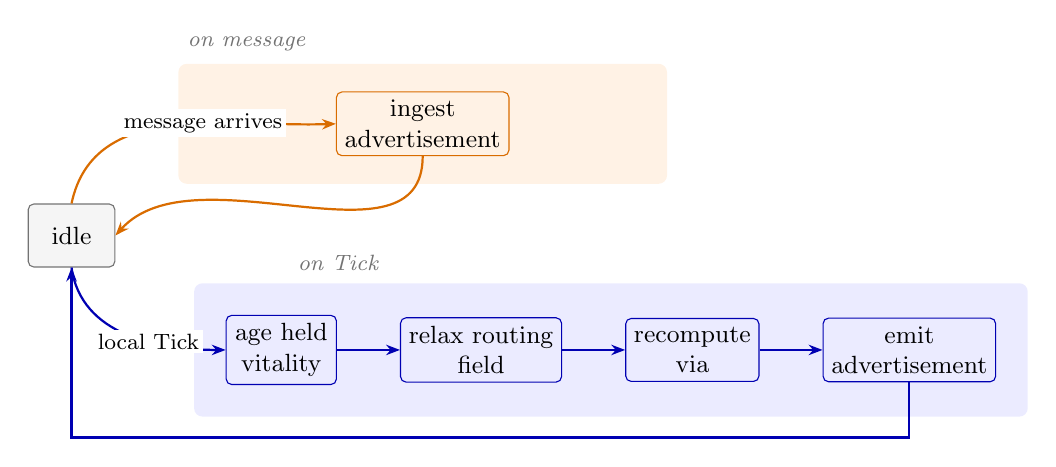
\begin{tikzpicture}[
  >={Stealth[length=5pt]},
  font=\small,
  node distance=10mm and 8mm,
  box/.style={rounded corners=2pt, draw, align=center, inner sep=3pt,
              minimum height=8mm, minimum width=14mm, text=black, fill=white},
  hub/.style={box, draw=black!55, fill=black!4, minimum width=11mm},
  recvbox/.style={box, draw=orange!85!black, fill=orange!10},
  emitbox/.style={box, draw=blue!70!black, fill=blue!8},
  recvedge/.style={draw=orange!85!black, ->, thick},
  emitedge/.style={draw=blue!70!black, ->, thick},
  elab/.style={font=\footnotesize, text=black, inner sep=1.5pt, fill=white},
  lanecap/.style={font=\footnotesize\itshape, text=black!55},
]
% --- hub (neutral, sits between the two lanes, in neither band) ---
\node[hub] (idle) {idle};

% --- top lane: reception ---
\node[recvbox, above right=6mm and 28mm of idle] (ingest) {ingest\\advertisement};

% --- bottom lane: emission ---
\node[emitbox, below right=6mm and 14mm of idle] (age) {age held\\vitality};
\node[emitbox, right=of age] (relax) {relax routing\\field};
\node[emitbox, right=of relax] (via) {recompute\\via};
\node[emitbox, right=of via] (emit) {emit\\advertisement};

% --- lane background bands (behind everything; bands DO NOT cover idle) ---
\begin{scope}[on background layer]
  \node[fill=orange!10, rounded corners=3pt, fit=(ingest),
        inner xsep=20mm, inner ysep=3.5mm] (recvband) {};
  \node[fill=blue!8, rounded corners=3pt, fit=(age)(emit),
        inner xsep=4mm, inner ysep=4mm] (emitband) {};
\end{scope}

% --- reception edges: short loop off idle (orange), the two arrows kept well apart ---
\draw[recvedge] (idle.north) to[out=78,in=182]
  node[elab, pos=0.6] {message arrives} (ingest.west);
\draw[recvedge] (ingest.south) to[out=-90,in=48,looseness=0.95] (idle.east);

% --- emission edges: long pipeline (blue) ---
\draw[emitedge] (idle.south) to[out=-82,in=180]
  node[elab, pos=0.62] {local Tick} (age.west);
\draw[emitedge] (age) -- (relax);
\draw[emitedge] (relax) -- (via);
\draw[emitedge] (via) -- (emit);
% return: drop into clear space below the band, run left, rise into idle.south
\coordinate (rdown) at ($(emit.south)+(0,-7mm)$);
\coordinate (rleft) at (idle.south |- rdown);
\draw[emitedge] (emit.south) -- (rdown) -- (rleft) -- (idle.south);

% --- lane captions: above each band's left edge, in clear space ---
\node[lanecap, anchor=south west] at ([yshift=1pt]recvband.north west) {on message};
\node[lanecap, anchor=south west] at ([xshift=12mm,yshift=1pt]emitband.north west) {on Tick};
\end{tikzpicture}

\caption{RING node cycle.  Message arrival and local cadence are independent event sources; the Tick is
an emission/aging cadence, not a route-expiry timer.}
\end{figure}

Adjacency is admitted by echo: neighbour $p$ contributes to the relaxation set
$N^{\leftrightarrow}(i)$ when $i$ hears $p$ and $p$'s advertisement lists $i$ in $\mathrm{Hears}$. Staleness
no longer cuts the field at a freshness window; it ages the link's conductance by (5.1a), so a silent
neighbour drains continuously. A received vitality is aged before adoption,
using one Tick of staleness per relay in the clock-free base protocol,
\[
V^d_i \leftarrow \max\!\Big(V^d_i,\operatorname{age}(V^d_p,1)\Big),
\]
while a node's held vitality is aged by its own elapsed local time.  A clock-synchronized deployment may
replace the fixed one-Tick relay cost by a measured transit time, but the base protocol never compares
clocks across nodes.

The data plane reads the RIB as a policy decision over two levels: the field floor says whether a
direction is known, and the vitality threshold says whether that direction is vouched for.

\begin{figure}[t]
\centering
% Forwarding decision (§7.1, hand-drawn — no data). The data plane reads the RIB as a two-level policy:
% field-known? then V>=phi?. Terminals are colour-coded by valence — forward (teal, positive),
% unreachable/drop (red), not-vouched/policy (amber); decision diamonds get a light blue fill; the
% yes/no edge labels are small rounded chips so they ride the edge mid-span, never touching a box.
% Baseline tikz libraries only (arrows.meta, positioning, shapes.geometric).
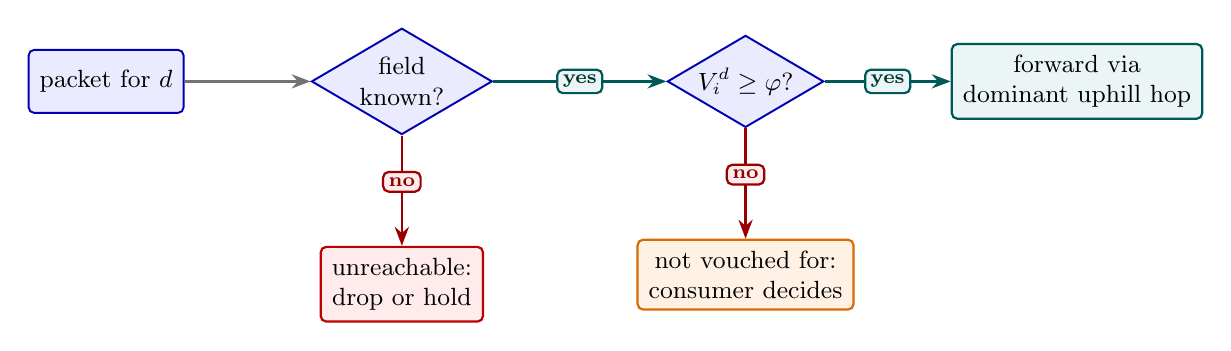
\begin{tikzpicture}[
  >={Stealth[length=2.4mm]},
  font=\small,
  node distance=10mm and 16mm,
  every node/.style={align=center},
  startnode/.style={
    rounded corners=2pt, draw=blue!70!black, fill=blue!8,
    text=black, inner sep=4pt, minimum height=8mm, line width=0.7pt},
  decision/.style={
    diamond, aspect=1.7, draw=blue!70!black, fill=blue!8,
    text=black, inner sep=1pt, line width=0.7pt},
  term/.style={
    rounded corners=2pt, text=black, inner sep=4pt,
    minimum height=8mm, line width=0.8pt},
  fwd/.style={term, draw=teal!70!black, fill=teal!8},
  drop/.style={term, draw=red!75!black, fill=red!8},
  policy/.style={term, draw=orange!85!black, fill=orange!10},
  yesedge/.style={->, draw=teal!70!black, line width=0.8pt},
  noedge/.style={->, draw=red!60!black, line width=0.8pt},
  plainedge/.style={->, draw=black!55, line width=0.8pt},
  yeschip/.style={
    fill=teal!8, draw=teal!70!black, text=teal!40!black,
    rounded corners=2pt, inner sep=2pt, font=\scriptsize\bfseries},
  nochip/.style={
    fill=red!8, draw=red!60!black, text=red!55!black,
    rounded corners=2pt, inner sep=2pt, font=\scriptsize\bfseries},
]
% --- nodes, left to right ---
\node[startnode] (pkt) {packet for $d$};
\node[decision, right=of pkt] (known) {field\\known?};

% known? --no--> drop (down), --yes--> vital (right)
\node[drop, below=14mm of known] (drop) {unreachable:\\drop or hold};
\node[decision, right=22mm of known] (vital) {$V^d_i\ge\varphi$?};

% vital? --yes--> fwd (right), --no--> policy (down)
\node[fwd, right=of vital] (fwd) {forward via\\dominant uphill hop};
\node[policy, below=14mm of vital] (policy) {not vouched for:\\consumer decides};

% --- edges ---
\draw[plainedge] (pkt) -- (known);

\draw[noedge] (known) -- node[nochip, pos=0.42] {no} (drop);
\draw[yesedge] (known) -- node[yeschip, pos=0.5] {yes} (vital);

\draw[yesedge] (vital) -- node[yeschip, pos=0.5] {yes} (fwd);
\draw[noedge] (vital) -- node[nochip, pos=0.42] {no} (policy);
\end{tikzpicture}

\caption{Forwarding decision.  Low vitality severs confidence, not direction; the caller chooses what to
do with a known but no-longer-vouched-for destination.}
\end{figure}

\section{Space–time horizon alignment and bounded state}\label{sec:spacetime}

There are two horizons and one stale-evidence clock. The routing field carries direction out to the spatial reach $\lambda\approx\sqrt{D/\kappa}$, set by the elliptic screening term $\kappa$. Vitality certifies liveness out to the policy action horizon
\[
R_V=\frac{1/\varphi-1}{\alpha},
\]
set by the proper-time aging rate $\alpha$ and the consumer's threshold $\varphi$. Link aging uses the same proper-time rate: if a separate symbol $\beta$ is introduced for stale conductance, the foundation chooses $\beta=\alpha$. The relationship between $\alpha$ and $\kappa$ is therefore a tuning relation, not an identity of mechanisms.

\textbf{Proposition 8.1 (bounded state).} If $\alpha$ is chosen so $R_V\asymp\lambda$, equivalently
\[
\alpha\asymp (1/\varphi-1)\sqrt{\kappa/D},
\tag{8.1}
\]
each node maintains non-negligible state only for destinations within an $O(\lambda)$ ball, so total fabric state is $O\!\big(n\cdot\mathrm{Vol}(\lambda)\big)$. \emph{Sketch.} Beyond $\lambda$ the screened field falls below the operational floor and the destination is not worth carrying as routing state (§\ref{sec:screened-balance}); aligning $R_V$ with $\lambda$ ensures vitality has likewise decayed below the policy threshold there. Each node's working set is its reach ball, of volume $\mathrm{Vol}(\lambda)$; summing over $n$ nodes gives the bound. $\;\square$

Exact equality $R_V=\lambda$ is only one regime. With $D=1$, $\kappa=0.05$, and $\varphi=0.5$, it corresponds to $\alpha=\sqrt{\kappa/D}\approx0.224$. A proving-ground deployment may instead keep the same $\kappa$-scaled aging rate while lowering the policy threshold, e.g. $\varphi=0.2$, which gives $R_V\approx4\lambda$: evidence ages on the field's scale, while the data plane is willing to act farther into the low-confidence tail. This is a policy choice over continuous fields, not a new foundation term.

This is the payoff of unifying space and time: the protocol natively snuffs out state for distant destinations rather than carrying global tables, and the locality radius can be exposed as a tuning relation among $\kappa$, $\alpha$, and $\varphi$. (Sub-$\mathrm{Vol}(\lambda)$ state would require hierarchy/landmarks, §\ref{sec:discussion}.)

\section{Empirical validation}\label{sec:empirical}

We validate the theory on the \emph{asynchronous} reference implementation: each node runs on its own cadence with no global round, barrier, or shared clock (§\ref{sec:operational}), and every measured figure is an ensemble of $R$ independent reps reported as a median with a 10--90\% inter-rep band. The exact-solve figures of §§\ref{sec:routing}--6 (\textsc{[exact]}) show what the operator \emph{defines}; the figures here (\textsc{[measured]}) show what the running protocol \emph{realizes}. This is a simulation study, not a deployment (§\ref{sec:discussion}); its purpose is to exercise each theorem on the live protocol.

\textbf{Lifecycle and the $V(\delta)$ droop.} A far observer converges, the source is killed, and its vitality severs gracefully through $\varphi$ to zero (Fig.~\ref{fig:timeseries}). Along a line the steady live $V$ tracks the law $1/(1+\alpha\delta)$ (Theorem 6.3) but ages slightly \emph{faster} than unit-transit predicts (Fig.~\ref{fig:vdroop}): a route also dwells in the RIB between refreshes, spending extra proper time. The measured-below-theory gap is that dwell, not error — the protocol is honest about evidence it has held longer than one hop's transit.

\begin{figure}[tbp]
\centering
% Vitality lifecycle at a far observer: converge, source killed, graceful severance through phi.
% Data: timeseries.dat (t_ms V phi), timeseries_kill.dat (vertical event segment). (figgen)
\providecommand{\figpath}{figures/}
\begin{tikzpicture}
\begin{axis}[
  width=\linewidth, height=6.2cm,
  xlabel={time (ms)}, ylabel={vitality $V$ at observer},
  xmin=0, xmax=4500, ymin=0, ymax=1.05,
  legend pos=north east, legend cell align=left,
  grid=both, grid style={black!8},
  tick align=outside, tick pos=left,
]
% action threshold
\addplot[draw=black!55, dashed, thick, mark=none] coordinates {(0,0.5) (4500,0.5)};
\addlegendentry{action threshold $\varphi$}
% source-kill event
\addplot[draw=red!70!black, dotted, very thick, mark=none]
  table[x=t, y=V] {\figpath timeseries_kill.dat};
\addlegendentry{source killed}
% measured vitality
\addplot[draw=blue!70!black, thick, mark=none, smooth]
  table[x=t, y=V] {\figpath timeseries.dat};
\addlegendentry{$V$ (measured)}
\end{axis}
\end{tikzpicture}

\caption{\textsc{[measured]} Vitality lifecycle at a far observer: the field converges, the source is killed (vertical mark), and the held vitality ages through the action threshold $\varphi$ to zero — graceful severance, no flap.}
\label{fig:timeseries}
\end{figure}

\begin{figure}[tbp]
\centering
% Measured field droop along a line vs. hop distance. Data: vdroop.dat (figgen).
\providecommand{\figpath}{figures/}
\begin{tikzpicture}
\begin{axis}[
  width=\linewidth, height=6.2cm,
  xlabel={hop distance $\delta$ from source},
  ylabel={field value toward source},
  xmin=0, xmax=8, ymin=0, ymax=1.05,
  xtick={0,1,...,8},
  legend pos=south west, legend cell align=left,
  grid=both, grid style={black!8},
  tick align=outside, tick pos=left,
]
\addplot[draw=black, dashed, thick, mark=none, samples at={0,...,8}]
  table[x=delta, y=Videal] {\figpath vdroop.dat};
\addlegendentry{$1/(1+\alpha\delta)$ (theory)}
\addplot[mark=square*, thick, red!75!black, mark options={scale=0.9}]
  table[x=delta, y=V] {\figpath vdroop.dat};
\addlegendentry{vitality $V$ (measured)}
\addplot[mark=*, thick, blue!70!black, mark options={scale=0.9}]
  table[x=delta, y=f] {\figpath vdroop.dat};
\addlegendentry{routing potential $f$ (measured)}
\end{axis}
\end{tikzpicture}

\caption{\textsc{[measured]} The $V(\delta)$ droop along a line: measured live vitality vs.\ hop distance tracks the unit-transit law $1/(1+\alpha\delta)$ (Theorem 6.3); the shaded gap is the protocol ageing $V$ slightly faster because a route also dwells in the RIB between refreshes — extra proper time, not error.}
\label{fig:vdroop}
\end{figure}

\textbf{Clock-free robustness.} Under unsynchronized clocks — per-node offsets up to $s$ ticks, either sign — the two retardation modes diverge (Fig.~\ref{fig:skew}). The clock-free hop-age (one tick of staleness per relay, never a cross-node clock read) is skew-invariant: it becomes routable while the source is live and severs after it dies in 100\% of reps at every skew. Reading a measured cross-clock transit instead — the NTP-dependent variant — degrades as the skew dwarfs the true sub-tick transit, over-ageing a live source below $\varphi$ or under-ageing a dead one: correctness falls to $0.71$ at $s=14$ and $0.48$ at $s=16$. Causal honesty needs no synchronized clock.

\begin{figure}[tbp]
\centering
% [MEASURED, async] Skew-robustness sweep. Under unsynchronized clocks (each node a random per-node
% offset of up to s Ticks, both signs, fresh pattern per rep), the two retardation modes diverge.
% Clock-free hop-age ages V by a fixed one Tick per relay and never reads a cross-node clock, so it is
% skew-invariant; measured cross-clock transit (recv_clock - emit_clock) needs NTP, and as the skew
% dwarfs the true sub-Tick transit it over-ages V below phi (a live source that never lights up) or
% under-ages it (a dead source that resurrects). TOP: fraction of reps that were CORRECT = (became
% routable while live) AND (severed after kill), R=21 reps per point. BOTTOM: steady live vitality V at
% the observer, median with a 10-90 percentile band. Data: skew.dat (figgen). Needs fillbetween.
\providecommand{\figpath}{figures/}
\begin{tikzpicture}
% --- TOP: fraction correct vs skew ---
\begin{axis}[
  name=frac,
  width=\linewidth, height=5.2cm,
  ylabel={fraction correct},
  xmin=0, xmax=16, ymin=0, ymax=1.05,
  xtick={0,2,...,16}, xticklabels={},
  ytick={0,0.25,0.5,0.75,1.0},
  legend pos=south west, legend cell align=left, legend style={font=\scriptsize},
  grid=both, grid style={black!8},
  tick align=outside, tick pos=left,
]
\addplot[draw=blue!70!black, thick, mark=*, mark options={scale=0.85}]
  table[x=skew, y=fracHop] {\figpath skew.dat};
\addlegendentry{clock-free hop-age (HopAge)}
\addplot[draw=red!75!black, thick, mark=square*, mark options={scale=0.85}]
  table[x=skew, y=fracMeas] {\figpath skew.dat};
\addlegendentry{measured transit (needs sync)}
\end{axis}
% --- BOTTOM: steady live vitality vs skew, median + 10-90 band ---
\begin{axis}[
  at={(frac.south west)}, anchor=north west, yshift=-0.85cm,
  width=\linewidth, height=5.2cm,
  xlabel={max per-node clock skew $s$ (Ticks)},
  ylabel={steady live $V$ at observer},
  xmin=0, xmax=16, ymin=0, ymax=1.0,
  xtick={0,2,...,16},
  legend pos=south west, legend cell align=left, legend style={font=\scriptsize},
  grid=both, grid style={black!8},
  tick align=outside, tick pos=left,
]
% action threshold phi
\addplot[draw=black!55, dashed, thick, mark=none] coordinates {(0,0.5) (16,0.5)};
\addlegendentry{action threshold $\varphi$}
% clock-free band + median
\addplot[name path=hopLo, draw=none, forget plot] table[x=skew, y=vLoHop] {\figpath skew.dat};
\addplot[name path=hopHi, draw=none, forget plot] table[x=skew, y=vHiHop] {\figpath skew.dat};
\addplot[blue!60!black, opacity=0.15, forget plot] fill between[of=hopLo and hopHi];
\addplot[draw=blue!70!black, thick, mark=*, mark options={scale=0.8}]
  table[x=skew, y=vMedHop] {\figpath skew.dat};
\addlegendentry{clock-free $V$ (median)}
% measured-transit band + median
\addplot[name path=measLo, draw=none, forget plot] table[x=skew, y=vLoMeas] {\figpath skew.dat};
\addplot[name path=measHi, draw=none, forget plot] table[x=skew, y=vHiMeas] {\figpath skew.dat};
\addplot[red!55!black, opacity=0.15, forget plot] fill between[of=measLo and measHi];
\addplot[draw=red!75!black, thick, mark=square*, mark options={scale=0.8}]
  table[x=skew, y=vMedMeas] {\figpath skew.dat};
\addlegendentry{measured $V$ (median)}
\end{axis}
\end{tikzpicture}
\caption{\textsc{[measured]} Skew-robustness sweep ($R=21$ reps/point). \emph{Top:} fraction of reps that are correct (routable while live \emph{and} severed after death); clock-free hop-age holds at $1$ across all skew, measured cross-clock transit degrades as skew dwarfs the true sub-tick transit. \emph{Bottom:} steady live $V$ at the observer (median, 10--90\% band) — skew-invariant for hop-age, scattered for measured-transit.}
\label{fig:skew}
\end{figure}

\textbf{Count-to-infinity, made graceful.} The headline contrast (Fig.~\ref{fig:dvring}, §\ref{sec:death}): on a dead line a textbook distance-vector metric counts upward to its cap while RING's reciprocal fade keeps the read $V$ bounded and monotone — the same diverging metric, read two ways. Retardation is what forbids the alternative pathology, the spurious resurrection that locks a dead source at $V=1$ (Fig.~\ref{fig:retardation}, §\ref{sec:retardation}).

\textbf{Data-plane delivery through failure.} On a converged grid every packet is delivered; a lossy fabric (4\%/hop) plateaus at $0.67$ delivered, the gap to one being physically lost mass, not a routing failure (Fig.~\ref{fig:blackhole}a). When the chokepoint directly above the destination is killed, delivery collapses to $0.09$ for one reconvergence window as stale routes forward into the corpse, and the black-hole ratio mirror-spikes to $0.91$ (Fig.~\ref{fig:blackhole}b). Then vitality ages the dead route past $\varphi$: forwarding cleanly \emph{severs} rather than black-holing, the field reconverges around the gap, and delivery snaps back to one.

\begin{figure}[tbp]
\centering
% The data-plane payoff, MEASURED from the async reference implementation (medians + bands over reps).
% (a) Delivery-latency CDF by hop count on a converged 12x10 grid toward a corner dst. Nominal reaches
%     1 (every packet delivered); the lossy fabric (4%/hop) plateaus at ~0.67 — the gap to 1 is the
%     physically-LOST mass (Lost), distinct from any routing failure. (b) A steady stream is injected;
%     at t0 the node directly above the dst — the chokepoint nearly all flow funnels through — is
%     killed. Delivery collapses to ~0.09 for one reconvergence window as stale routes forward INTO the
%     corpse (BlackholeDeadHop); the black-hole ratio mirror-spikes to ~0.90 (both are fractions of the
%     injected packets, so they share one [0,1] axis and sum to ~1 in the stale window). Then vitality
%     ages the dead route past φ, forwarding cleanly SEVERS (not a black hole), and the field
%     reconverges around the gap: delivery snaps back to 1 and black-holes fall to zero. The band is the
%     p25..p75 spread over reps — the async reconvergence instant jitters, so the recovery window
%     straddles. Data: blackhole_cdf_{nominal,lossy}.dat, blackhole_ts.dat, blackhole_ts_kill.dat
%     (figgen). Needs fillbetween.
\providecommand{\figpath}{figures/}
\begin{tikzpicture}

% ---- (a) delivery-latency CDF -------------------------------------------------------------------
\begin{axis}[
  name=cdf,
  width=6.2cm, height=4.4cm, scale only axis,
  xlabel={delivery hops}, ylabel={CDF (delivered fraction)},
  xmin=0, xmax=20, ymin=0, ymax=1.02,
  legend pos=south east, legend cell align=left, legend style={font=\scriptsize},
  grid=both, grid style={black!8}, tick align=outside, tick pos=left,
  title={(a) delivery-latency CDF}, title style={font=\small},
]
\addplot[draw=blue!70!black, thick, const plot, mark=none]
  table[x=hops, y=cdf] {\figpath blackhole_cdf_nominal.dat};
\addlegendentry{nominal (lossless)}
\addplot[draw=orange!85!black, thick, const plot, mark=none]
  table[x=hops, y=cdf] {\figpath blackhole_cdf_lossy.dat};
\addlegendentry{lossy ($4\%$/hop)}
% the lost mass: the gap between the lossy plateau and 1.
\addplot[draw=orange!60!black, dashed, mark=none]
  coordinates {(0,0.670972) (20,0.670972)};
\addlegendentry{lossy plateau (= delivered)}
\node[anchor=south east, font=\scriptsize, orange!60!black] at (axis cs:20,0.69) {lost mass $\uparrow$};
\end{axis}

% ---- (b) delivery-ratio + black-hole-ratio timeseries across the kill ----------------------------
% ONE [0,1] axis: delivery ratio and black-hole ratio (fraction of injected packets) are both rates,
% so they share a frame — no fragile twin-axis alignment. During the stale window they sum to ~1:
% almost every packet that is not delivered is black-holed (stale route INTO the corpse). Once
% vitality severs, both fall to their floors as forwarding cleanly declines (Severed, off-figure).
\begin{axis}[
  name=ts,
  at={(cdf.south east)}, anchor=south west, xshift=2.0cm,
  width=6.2cm, height=4.4cm, scale only axis,
  xlabel={time (ms)}, ylabel={fraction of injected packets},
  xmin=0, xmax=1100, ymin=0, ymax=1.05,
  legend style={at={(0.97,0.5)}, anchor=east, font=\scriptsize}, legend cell align=left,
  grid=both, grid style={black!8}, tick align=outside, tick pos=left,
  title={(b) delivery \& black-holes through a node death}, title style={font=\small},
]
% kill marker
\addplot[draw=red!70!black, dotted, very thick, mark=none]
  table[x=t, y=v] {\figpath blackhole_ts_kill.dat};
\addlegendentry{node killed}
% delivery-ratio band (p25..p75) + median
\addplot[name path=drLo, draw=none, forget plot] table[x=t_ms, y=drLo] {\figpath blackhole_ts.dat};
\addplot[name path=drHi, draw=none, forget plot] table[x=t_ms, y=drHi] {\figpath blackhole_ts.dat};
\addplot[blue!60!black, opacity=0.15, forget plot] fill between[of=drLo and drHi];
\addplot[draw=blue!70!black, thick, mark=*, mark options={scale=0.6}]
  table[x=t_ms, y=deliveryRatio] {\figpath blackhole_ts.dat};
\addlegendentry{delivery ratio (median)}
% black-hole-ratio band (p25..p75) + median
\addplot[name path=brLo, draw=none, forget plot] table[x=t_ms, y=bhrLo] {\figpath blackhole_ts.dat};
\addplot[name path=brHi, draw=none, forget plot] table[x=t_ms, y=bhrHi] {\figpath blackhole_ts.dat};
\addplot[red!60!black, opacity=0.12, forget plot] fill between[of=brLo and brHi];
\addplot[draw=red!75!black, thick, dashed, mark=*, mark options={scale=0.6}]
  table[x=t_ms, y=bhRatio] {\figpath blackhole_ts.dat};
\addlegendentry{black-hole ratio (median)}
\end{axis}

\end{tikzpicture}
\caption{\textsc{[measured]} The data-plane payoff. (a) Delivery-latency CDF by hop count on a converged grid: nominal reaches $1$ (every packet delivered); the lossy fabric (4\%/hop) plateaus at $0.67$, the gap being physically lost mass, distinct from any routing failure. (b) A steady stream is injected and the chokepoint above the destination is killed at $t_0$: delivery collapses to $0.09$ and the black-hole ratio mirror-spikes to $0.91$ for one reconvergence window (they sum to $\approx\!1$ over the injected packets), then vitality severs the dead route and delivery snaps back to $1$.}
\label{fig:blackhole}
\end{figure}

\textbf{Partition and recovery.} Cutting the only bridge on a line collapses delivery (Fig.~\ref{fig:partition}). The black-hole fraction spikes first — stale field routing packets into the dead edge — then hands off to correct severance as vitality ages below $\varphi$: the protocol declining to forward, not a black hole. After the heal the field reconverges and delivery recovers within $\sim\!100$~ms.

\begin{figure}[tbp]
\centering
% Partition + recovery on a line (bridge edge CUT then RELINKED), MEASURED from the async reference
% implementation as an ensemble over R=21 reps (delivery ratio = delivered/(reps·pkts), min/max band).
% Top axis: data-plane delivery ratio collapses at the cut and recovers ~100 ms after the heal; the
% black-hole fraction (stale field routing packets into the dead edge — a transient via-cycle) spikes
% first, then hands off to correct SEVERANCE (routable→0, bottom axis) as vitality ages below φ — the
% protocol declining to forward, NOT a black hole. Markers are the measured cut / heal / recovered
% instants (partition_events.dat). Data: partition.dat. Needs fillbetween.
\providecommand{\figpath}{figures/}
\begin{tikzpicture}
\begin{axis}[
  name=top,
  width=\linewidth, height=5.4cm,
  xlabel={}, xticklabels={},
  ylabel={fraction of packets},
  xmin=-120, xmax=1200, ymin=-0.03, ymax=1.08,
  ytick={0,0.25,0.5,0.75,1},
  legend style={at={(0.42,0.55)}, anchor=west}, legend cell align=left, legend style={font=\scriptsize, fill=white, fill opacity=0.85, text opacity=1},
  grid=both, grid style={black!8},
  tick align=outside, tick pos=left,
]
% event markers (measured instants): cut at 0, heal at 700, recovered at 800
\draw[red!70!black, dotted, very thick] (axis cs:0,-0.03) -- (axis cs:0,1.08);
\draw[green!45!black, dotted, very thick] (axis cs:700,-0.03) -- (axis cs:700,1.08);
\draw[green!45!black, dashed, thick] (axis cs:800,-0.03) -- (axis cs:800,1.08);
\node[red!70!black, font=\scriptsize\bfseries, anchor=south, rotate=90] at (axis cs:0,0.18) {cut};
\node[green!45!black, font=\scriptsize\bfseries, anchor=south, rotate=90] at (axis cs:700,0.18) {relink};
\node[green!45!black, font=\scriptsize, anchor=west] at (axis cs:805,0.55) {recovered $+100$\,ms};
% delivery min/max band over reps
\addplot[name path=lo, draw=none, forget plot] table[x=t, y=delivLo] {\figpath partition.dat};
\addplot[name path=hi, draw=none, forget plot] table[x=t, y=delivHi] {\figpath partition.dat};
\addplot[blue!60!black, opacity=0.14] fill between[of=lo and hi];
\addlegendentry{delivery band (reps)}
% black-hole fraction (transient via-cycle into the dead edge)
\addplot[draw=red!75!black, thick, mark=none] table[x=t, y=black] {\figpath partition.dat};
\addlegendentry{black-holed (stale field)}
% delivery ratio (ensemble mean)
\addplot[draw=blue!70!black, very thick, mark=none] table[x=t, y=deliv] {\figpath partition.dat};
\addlegendentry{delivered}
\end{axis}
\begin{axis}[
  at={(top.south west)}, anchor=north west, yshift=-0.55cm,
  width=\linewidth, height=3.2cm,
  xlabel={time since cut (ms)}, ylabel={far side},
  xmin=-120, xmax=1200, ymin=-0.12, ymax=1.12,
  ytick={0,1}, yticklabels={severed, routable},
  legend pos=south east, legend cell align=left, legend style={font=\scriptsize, fill=white, fill opacity=0.85, text opacity=1},
  grid=both, grid style={black!8},
  tick align=outside, tick pos=left,
]
\draw[red!70!black, dotted, very thick] (axis cs:0,-0.12) -- (axis cs:0,1.12);
\draw[green!45!black, dotted, very thick] (axis cs:700,-0.12) -- (axis cs:700,1.12);
\draw[green!45!black, dashed, thick] (axis cs:800,-0.12) -- (axis cs:800,1.12);
% routable fraction across reps, as a step (control-plane state)
\addplot[draw=black!80, very thick, const plot, mark=none] table[x=t, y=routable] {\figpath partition.dat};
\addlegendentry{routable fraction}
% severed fraction overlaid (correct declination, not a black hole)
\addplot[draw=orange!80!black, thick, dashed, const plot, mark=none] table[x=t, y=sever] {\figpath partition.dat};
\addlegendentry{severed (correct)}
\end{axis}
\end{tikzpicture}
\caption{\textsc{[measured]} Partition and recovery on a line ($R=21$ reps). The bridge edge is cut, then relinked. Data-plane delivery (top) collapses at the cut and recovers $\sim\!100$~ms after the heal; the black-hole fraction spikes first, then hands off to correct severance (routable$\to 0$, bottom) as vitality ages below $\varphi$. Markers are the measured cut / heal / recovered instants.}
\label{fig:partition}
\end{figure}

\textbf{Link-aging reroutes around dead relays.} A dead \emph{relay} on a redundant path is the case neither $\kappa$ nor vitality handles (§\ref{sec:stale-evidence}): the destination stays live via the backup, so vitality never severs, yet the relay's frozen advertisement would pin the field onto the corpse. On a diamond — a preferred 2-hop relay and a longer 3-hop backup — we kill the preferred relay and read delivery over time (Fig.~\ref{fig:linkaging}). Without link-aging (the \texttt{NoLinkAge} ablation) delivery stays at zero, a permanent black hole. With it, the dead link's conductance drains as the reciprocal $1/g^{\mathrm{eff}}=1/g+\alpha k$ — matching the ideal to the digit — while live links hold near $g$ with a bounded sawtooth; once the corroding link falls below the backup, the field reroutes and delivery snaps to one. The dead-relay drain of §\ref{sec:stale-evidence}, measured: failure detection by the same proper-time operator that ages vitality, with no freshness timer.

\begin{figure}[tbp]
\centering
% Link-aging reroutes around a dead RELAY on its own (§5.4), measured on the diamond at the illustrative
% α=0.04: a preferred 2-hop path src-a-dst and a longer 3-hop backup src-b1-b2-dst; the relay `a` is
% killed at t=0. The destination stays alive via the backup, so vitality toward it never severs — only
% the aged link conductance can reroute. TOP: delivery fraction after the kill — the NoLinkAge ablation
% (freeze: a's frozen potential is a permanent pin, delivery stays 0) vs the foundation (aged: a's link
% drains and the field reroutes, delivery recovers to 1). BOTTOM: the effective conductance — the dead
% link draining as the reciprocal 1/g_eff = 1/g + αk (coinciding with the ideal overlay) and a live link
% holding near g (a bounded sawtooth). Data: linkaging_delivery.dat, linkaging_drain.dat.
\providecommand{\figpath}{figures/}
\begin{tikzpicture}
\begin{axis}[
  name=del,
  width=\linewidth, height=4.8cm,
  xlabel={time after the relay is killed (ms)}, ylabel={delivery fraction},
  xmin=0, xmax=3550, ymin=-0.05, ymax=1.10,
  xtick={0,500,1000,1500,2000,2500,3000,3500}, x tick label style={/pgf/number format/1000 sep={}},
  legend pos=south east, legend cell align=left, legend style={font=\scriptsize},
  grid=both, grid style={black!8}, tick align=outside, tick pos=left,
]
\addplot[draw=red!75!black, very thick, mark=none]
  table[x=t, y=freeze] {\figpath linkaging_delivery.dat};
\addlegendentry{no link-aging (freeze): permanent black hole}
\addplot[draw=teal!65!black, very thick, mark=none]
  table[x=t, y=aged] {\figpath linkaging_delivery.dat};
\addlegendentry{link-aging: the field reroutes}
\node[anchor=west, font=\scriptsize, teal!45!black] at (axis cs:1050,0.55) {dead link drained enough $\Rightarrow$ reroute};
\end{axis}

\begin{axis}[
  at={(del.south west)}, anchor=north west, yshift=-1.4cm,
  width=\linewidth, height=4.8cm,
  xlabel={time after the relay is killed (ms)}, ylabel={effective conductance $g^{\mathrm{eff}}$},
  xmin=0, xmax=3550, ymin=0, ymax=1.10,
  xtick={0,500,1000,1500,2000,2500,3000,3500}, x tick label style={/pgf/number format/1000 sep={}},
  legend pos=north east, legend cell align=left, legend style={font=\scriptsize},
  grid=both, grid style={black!8}, tick align=outside, tick pos=left,
]
\addplot[draw=teal!65!black, very thick, mark=none]
  table[x=t, y=g_dead] {\figpath linkaging_drain.dat};
\addlegendentry{dead link $a$ (measured): $1/g^{\mathrm{eff}}=1/g+\alpha k$}
\addplot[draw=black!55, densely dashed, line width=0.9pt, mark=none]
  table[x=t, y=g_ideal] {\figpath linkaging_drain.dat};
\addlegendentry{ideal $1/(1+\alpha k)$ (overlaid)}
\addplot[draw=orange!85!black, thick, mark=none]
  table[x=t, y=g_live] {\figpath linkaging_drain.dat};
\addlegendentry{live link $b_1$: bounded sawtooth}
\end{axis}
\end{tikzpicture}

\caption{\textsc{[measured]} Link-aging reroutes around a dead relay (§\ref{sec:stale-evidence}), on a diamond with a preferred 2-hop relay $a$ and a longer 3-hop backup, at the illustrative $\alpha=0.04$. \emph{Top:} delivery after $a$ is killed — without link-aging (the \texttt{NoLinkAge} ablation) the frozen potential is a permanent pin and delivery stays at zero; with it the field reroutes and delivery recovers to one once the dead link has drained. \emph{Bottom:} the dead link's effective conductance draining as the reciprocal $1/g^{\mathrm{eff}}=1/g+\alpha k$ (coinciding with the ideal $1/(1+\alpha k)$), while a live link holds near $g$ with a bounded sawtooth.}
\label{fig:linkaging}
\end{figure}

\textbf{Loop-dissipativity under churn.} Snapshotting the forwarding via-graph on a skewed, thrice-churned mesh and DFS-counting its directed cycles, transient via-cycles flicker as the field re-grows on stale advertisements — at most three at once, mean length $\approx 1.2$ hops — and every one dissipates to zero within a few rounds; none persists (Theorem 5.7, Fig.~\ref{fig:loops}). Kills collapse the field monotonically and raise no loop; only revives spark a transient.

\begin{figure}[tbp]
\centering
% Loop-dissipativity under async churn (Thm 5.7, measured on the reference implementation). Read-only
% over the live mesh: at each sample we snapshot every node's forwarding via toward a fixed source,
% build the directed via-graph, and DFS-count its directed cycles — the transient forwarding loops.
% The mesh is skewed (out-of-step clocks) and churned (interior killed, then revived, three rounds).
% Transient via-cycles flicker into existence as the field re-grows and adjacent nodes momentarily
% cross on stale advertisements, then DISSIPATE to 0 within a few rounds — they never persist (the
% screened potential is a discrete subharmonic with no spurious interior maximum). Kills collapse the
% field monotonically and raise no loop; only revives spark the spike. Measured: median+envelope over
% R=21 async reps. Data: loops.dat (t mean p90 max maxlen), loops_kill/revive.dat (event instants).
% Needs \usepgfplotslibrary{fillbetween}.
\providecommand{\figpath}{figures/}
\begin{tikzpicture}
\begin{axis}[
  width=\linewidth, height=6.2cm,
  xlabel={time (ms)}, ylabel={transient via-cycles},
  xmin=0, xmax=6200, ymin=0, ymax=5.4,
  ytick={0,1,2,3,4,5},
  legend pos=north west, legend cell align=left, legend style={font=\scriptsize},
  grid=both, grid style={black!8},
  tick align=outside, tick pos=left,
]
% disturbance markers: kills (grey, monotone collapse, no loop) and revives (red, the spike)
\addplot[draw=black!45, dotted, very thick, mark=none]
  table[x=t, y expr=\thisrow{y}*5.4] {\figpath loops_kill.dat};
\addlegendentry{interior killed}
\addplot[draw=red!70!black, dotted, very thick, mark=none]
  table[x=t, y expr=\thisrow{y}*5.4] {\figpath loops_revive.dat};
\addlegendentry{interior revived}
% max envelope over reps (worst-case simultaneous loops), shaded to the axis
\addplot[name path=maxenv, draw=blue!30, thick, mark=none, const plot]
  table[x=t, y=max] {\figpath loops.dat};
\addplot[name path=zero, draw=none, mark=none] table[x=t, y expr=0] {\figpath loops.dat};
\addplot[blue!55, opacity=0.14] fill between[of=maxenv and zero];
\addlegendentry{max over reps (envelope)}
% mean cycle count per snapshot (the central statistic): spikes at each revive, decays to 0
\addplot[draw=blue!75!black, very thick, mark=none]
  table[x=t, y=mean] {\figpath loops.dat};
\addlegendentry{mean cycles / snapshot}
\end{axis}
\end{tikzpicture}

\caption{\textsc{[measured]} Loop-dissipativity under async churn (Theorem 5.7). At each sample the forwarding via-graph is snapshotted and its directed cycles DFS-counted, read-only over a skewed, thrice-churned mesh. Transient via-cycles flicker as the field re-grows on stale advertisements (at most three at once, mean length $\approx 1.2$ hops) and dissipate to zero within a few rounds; none persists. Kills raise no loop — only revives spark a transient. Median $+$ envelope over $R=21$ reps.}
\label{fig:loops}
\end{figure}

\textbf{Congestion damping.} On a barbell whose single bridge carries all cross-cluster current, the hub self-measures that load and glides its screening charge $\mu$ toward $c\,s$ with no injected stress (Fig.~\ref{fig:congestion}, top). The charge climbs monotonically to its equilibrium $\mu^\star=c\,s(\mu^\star)$ with no overshoot — the non-overshoot integrator's damped settle (Lemma 5.8). The loop stays monotone-stable at \emph{every} coupling we tested (to $c=32$): the up-gradient load saturates ($s\to s_\infty\!\approx\!4$), so the realized single-node loop gain $\gamma_{\mathrm{loop}}(c)=c\,s'(\mu^\star)$ measured at the operating point holds far below the $\gamma_{\mathrm{loop}}=1$ threshold and \emph{falls} as $c$ rises ($0.40$ at the lightest load, $0.06$ at $c=1$, $0.002$ at $c=32$); a naive fixed light-load slope would predict the gain crossing $1$, but saturation defeats it (Fig.~\ref{fig:congestion}, bottom). We observe no instability boundary — the energy bound $\lambda_{\max}(\operatorname{Sym}J)<1$ (Theorem 5.9) holds throughout, even though the per-node self-term $\partial s_i/\partial\mu_i\ge0$ is non-dissipative (§\ref{sec:congestion}, Appendix C.5).

\begin{figure}[tbp]
\centering
% The self-driven load↔charge loop and its stability basin (Thm 5.9), measured on a barbell: two
% cliques joined by ONE bridge edge, so all cross-cluster current funnels through the bridge hub, which
% self-measures that load and glides its screening charge µ toward Crowd·load — no injected stress, the
% loop is internal. TOP: the hub's charge trajectory at the three named couplings, normalised to each
% curve's own equilibrium µ∞, so they overlay; every curve climbs monotonically to 1 with no overshoot
% — the damped settle the non-overshoot integrator guarantees inside the basin. BOTTOM: a wide coupling
% sweep of the transient overshoot (peak µ above µ∞, %), median + 10–90 band over reps; flat through the
% named couplings (wide basin) and lifting off only once the gain amplifies the convergence load-spike —
% the basin boundary made empirical. Measured from the reference implementation (median over reps, async).
% Data: congestion_ts.dat, congestion_basin.dat. Needs \usepgfplotslibrary{fillbetween}.
\providecommand{\figpath}{figures/}
\begin{tikzpicture}
\begin{axis}[
  name=ts,
  width=\linewidth, height=5.4cm,
  xlabel={time (ms)}, ylabel={charge $\mu/\mu_\infty$ (bridge)},
  xmin=0, xmax=2400, ymin=0, ymax=1.12,
  legend pos=south east, legend cell align=left, legend style={font=\scriptsize},
  grid=both, grid style={black!8},
  tick align=outside, tick pos=left,
]
% equilibrium reference
\addplot[draw=black!55, dashed, thick, mark=none] coordinates {(0,1) (2400,1)};
\addlegendentry{equilibrium $\mu_\infty$}
\addplot[draw=blue!70!black, thick, mark=none, smooth]
  table[x=t, y=n0p3] {\figpath congestion_ts.dat};
\addlegendentry{$c=0.3$ (deep in basin)}
\addplot[draw=teal!70!black, thick, mark=none, smooth]
  table[x=t, y=n1] {\figpath congestion_ts.dat};
\addlegendentry{$c=1.0$}
\addplot[draw=orange!85!black, thick, mark=none, smooth]
  table[x=t, y=n2] {\figpath congestion_ts.dat};
\addlegendentry{$c=2.0$}
\end{axis}

\begin{axis}[
  at={(ts.south west)}, anchor=north west, yshift=-1.55cm,
  width=\linewidth, height=5.0cm,
  xlabel={congestion coupling $c$ (\texttt{Crowd})},
  ylabel={transient overshoot of $\mu$ (\%)},
  xmode=log, log basis x=2,
  xmin=0.25, xmax=28, ymin=-1, ymax=30,
  legend pos=north west, legend cell align=left, legend style={font=\scriptsize},
  grid=both, grid style={black!8},
  tick align=outside, tick pos=left,
]
% 10–90 band over reps
\addplot[name path=lo, draw=none, forget plot] table[x=crowd, y=over_lo] {\figpath congestion_basin.dat};
\addplot[name path=hi, draw=none, forget plot] table[x=crowd, y=over_hi] {\figpath congestion_basin.dat};
\addplot[red!55!black, opacity=0.18] fill between[of=lo and hi];
\addlegendentry{10--90 band (reps)}
% median overshoot
\addplot[draw=red!75!black, thick, mark=*, mark options={scale=0.7}]
  table[x=crowd, y=over_med] {\figpath congestion_basin.dat};
\addlegendentry{median overshoot}
% the named couplings sit in the flat, damped floor
\addplot[only marks, mark=o, mark options={scale=1.6, draw=blue!70!black, line width=0.7pt}]
  coordinates {(0.3,0.27) (1.0,0.04) (2.0,0.02)};
\addlegendentry{named couplings (damped)}
\node[anchor=south, font=\scriptsize, black!60] at (axis cs:0.7,2.0) {basin floor};
\node[anchor=west, font=\scriptsize, red!60!black] at (axis cs:9,18) {ringing};
\end{axis}
\end{tikzpicture}

\caption{\textsc{[measured]} The self-driven load$\leftrightarrow$charge loop (§\ref{sec:congestion}–§\ref{sec:congestion-stability}) on a barbell bridge. \emph{Top:} the hub's charge at three couplings, each normalised to its own equilibrium $\mu_\infty$; every curve climbs monotonically to $1$ with no overshoot — the non-overshoot integrator's damped settle (Lemma 5.8). \emph{Bottom:} the realized single-node loop gain $\gamma_{\mathrm{loop}}(c)=c\,s'(\mu^\star)$ at the operating point $\mu^\star=c\,s(\mu^\star)$, swept over coupling. Because the up-gradient load saturates ($s'\!\to\!0$ as $\mu$ grows), the realized gain (solid) stays far below the $\gamma_{\mathrm{loop}}=1$ instability threshold at every coupling and falls as $c$ rises — no instability boundary. The naive gain a fixed light-load slope predicts (dashed) shoots past $1$; saturation defeats it.}
\label{fig:congestion}
\end{figure}

Together these exercise every theorem of §§\ref{sec:routing}--6 on the running protocol. The exact fields of §§\ref{sec:routing}--6 are what the operator defines; the ensembles here are what an asynchronous, clock-free implementation delivers.

\section{Discussion and limitations}\label{sec:discussion}

\textbf{Idealizations.} The clean $V(\delta)=1/(1+\alpha\delta)$ assumes unit per-hop transit; the general result is $V=1/(1+\alpha T)$ with $T$ the least accumulated transit time, which is what a deployment with heterogeneous link delay realizes. Closed-loop congestion stability is \emph{proven}, not empirical (Theorem 5.9): because the fields are exact, the load–charge loop is an exact map, globally ring-free whenever the loop gain stays below one. In the deployed loop that bound is met with room to spare — the up-gradient load saturates, so the realized gain stays far below one at every coupling and the loop is monotone-stable throughout (§\ref{sec:empirical}, Appendix C.5) — while a closed-form threshold for the multi-node map when the gain exceeds one remains open.

\textbf{Control-plane cost.} Liveness requires the source's assertion to be refreshed; a per-tick keepalive of the live working set is the simplest realization and is not silent at rest. It can be slowed to a lazy pulse at the cost of detection latency — a bandwidth/latency trade governed by $\alpha$ and the keepalive period.

\textbf{Scope.} Proposition 8.1 bounds state to a reach ball; genuinely sub-$\mathrm{Vol}(\lambda)$ routing (internet-scale diameters) needs hierarchy or landmarks layered above the field, which we do not address. The asynchronous shortest-path convergence of (6.2) is invoked, not reproved. The relationship between the discrete operators and the continuum PDEs — formerly stated by analogy — is made precise in Appendix B: on the fabric both fields are \emph{exact} discrete objects (a linear M-matrix solve and a min-plus shortest path), and the elliptic screened-Poisson and eikonal equations govern them only under a monotone–consistent–stable manifold-discretization limit (Barles and Souganidis 1991; Calder and Ettehad 2022) whose sampling hypotheses a logical fabric does not satisfy — and against which a naive graph distance is metrication-biased. We therefore do \emph{not} claim the deployed network is governed by a PDE, only that its discrete fields are the exact combinatorial objects those PDEs idealize.

\textbf{Future work.} A kernel data plane carrying the two scalars as the only per-destination state — programming the forwarding table over netlink and forwarding in eBPF, exposed as a CNI plugin for container fabrics — with conductance and transit measured from the link rather than assumed uniform; hierarchical aggregation beyond the reach ball; and a closed-form threshold for the multi-node congestion loop beyond gain one — bracketed in Appendix C.5 between the conservative $\lambda_{\max}(\operatorname{Sym}J)<1$ and the saturated $\rho(c\,Ds)=1$, but still open.

\section{Conclusion}\label{sec:conclusion}

RING maps the heuristic machinery of distributed routing — metrics, timers, sequence numbers, tombstones, hold-downs — onto two \emph{exact} discrete fields solved by local asynchronous iteration. Direction is the exact solution of a screened M-matrix system whose maximum principle makes forwarding loop- and black-hole-free; confidence is the exact proper-time shortest path whose reciprocal turns count-to-infinity into graceful death. The two share one screening charge that also absorbs congestion, and the elliptic and eikonal equations a physicist would write for them are their continuum shadows (Appendix B), not the equations the fabric solves. What remains is a fabric bent by load and aged by proper time, carrying packets down the steepest gradient — no telecom algorithms left.

\appendix
\section{Supplementary detail}

\textbf{A.1 The M-matrix properties (§\ref{sec:notation}).} $\mathcal{L}_g$ has non-positive off-diagonals $-g_{ij}$ and row sums zero; adding $Q\succ0$ yields strict row diagonal dominance $G_i+q_i>G_i=\sum_{j}|{-g_{ij}}|$. A symmetric, strictly diagonally dominant matrix with non-positive off-diagonals and positive diagonal is a Stieltjes (symmetric M-) matrix: positive-definite, with real positive eigenvalues and an entrywise non-negative inverse (Berman and Plemmons 1994; Varga 1962). Inverse-positivity gives $f^{d\star}\ge 0$ for the non-negative boundary data of (5.1), and strict positivity on $d$'s connected component.

\textbf{A.2 Domination of the self-term in (6.2).} The reciprocal update carries a self-term $U^d_i+\alpha$ (the node aging in the absence of fresher news). Since $U^d_i+\alpha>U^d_i\ge\min_j(U^d_j+\alpha\tau_{ij})$ whenever a live path exists, the self-term never attains the min at a live destination and the fixed point is the pure Bellman value $1+\alpha T^d_i$. With \emph{no} live source the self-term is the only term and drives $U\to\infty$ — the death dynamics of §\ref{sec:death}.

\textbf{A.3 Asynchronous shortest-path convergence of (6.2).} The min-plus operator $T(U)_i=\min_j(U^d_j+ \alpha\tau_{ij})$ is monotone and a (weighted) contraction toward the unique solution with non-negative weights and a fixed source value; the asynchronous convergence of such Bellman iterations under bounded communication and computation delay is classical (Bertsekas 1982; Bertsekas and Tsitsiklis 1989). The reciprocal $V=1/U$ inherits convergence by continuity away from $U=\infty$.

\textbf{A.4 Loop-dissipativity round bound.} In Theorem 5.7, the convergence rate fixes the window: samples fall within $g_{\min}/2$ of equilibrium after $O\!\big(\log(C/g_{\min})/\log(1/\gamma)\big)$ rounds, with $C$ the initial discrepancy and $g_{\min}$ the least nonzero equilibrium gap; thereafter only level-set circulation (vanishing current) remains.

\section{The exact discrete fields and their continuum limits}

The body names $f$ an "elliptic screened-Poisson potential" and $U=1/V$ an "eikonal" field. This appendix makes both names precise and, equally, bounds them. On the fabric \emph{both} fields are \textbf{exact} discrete objects, computed with no limit; the named partial differential equations are their \emph{shared continuum limits}, which a logical fabric is not built to take. We state the exact claims (B.1, B.2), the limit (B.3), and the scope (B.4).

\textbf{B.1 The vitality field is an exact discrete eikonal.} Fix a live destination $d$ ($U_d=1$), transit times $\tau_{ij}\ge 1$, aging rate $\alpha>0$, weights $w_{ij}=\alpha\tau_{ij}>0$. The min-plus relation (6.2) is the Bellman optimality equation of the shortest-path problem with these weights; on the component that can reach $d$, the strictly positive weights forbid zero/negative cycles, so it has the \textbf{unique finite solution}

\[
U^d_i = 1 + \alpha\, T^d_i,\qquad T^d_i=\min_{P:\,d\rightsquigarrow i}\ \sum_{(j,k)\in P}\tau_{jk},
\]

the least-accumulated-proper-time metric (Bellman 1958; Bertsekas 1982; Bertsekas and Tsitsiklis 1989). This is exact — a combinatorial optimum, no mesh and no limit. The operator $(\mathsf T U)_i=\min_{j\in N(i)}(U_j+\alpha\tau_{ij})$ is \textbf{monotone} (order-preserving), and its iteration is asynchronous Bellman–Ford; it converges by monotone dynamic programming, \emph{not} by a sup-norm contraction (that is the routing field's mechanism, §\ref{sec:convergence}). Over the $(\min,+)$ tropical (idempotent) semiring the operator is \textbf{linear} — the fixed point is the Kleene star $U=W^{*}\!\otimes b$, finite because $\tau_{ij}\ge 1$ excludes non-positive cycles (Litvinov 2005). The reciprocal $V=1/U$ is thus an \emph{exact} linearization of the nonlinear retarded-max update (6.1) into this tropically-linear problem; the Cole–Hopf transform (Hopf 1950; Cole 1951) is its continuum analogue, not its mechanism.

\textbf{B.2 The routing field is an exact discrete screened operator.} The relation (5.1) is the row equation of the finite linear system $(\mathcal{L}_g+Q)f^d=0$ with $f^d_d=F_0$. Because $\mathcal{L}_g+Q$ is a symmetric M-matrix (§\ref{sec:notation}), it is invertible with a non-negative inverse, so $f^d$ is the \textbf{exact, unique} solution — again no mesh, no limit — and the reach $\lambda$, the maximum principle, and the contraction (Lemma 5.1) are exact statements about this discrete operator. The "screened-Poisson" / Helmholtz \emph{PDE} $-D\nabla^2 f+\kappa f=0$ is its continuum limit (B.3), not its definition.

\textbf{B.3 The continuum limits, and their hypotheses.} Both PDEs are recovered only when the graph discretizes an underlying length space or manifold, with edge data approximating the metric and a sampling/bandwidth scale driven to zero. The abstract bridge is Barles and Souganidis (1991): a \emph{monotone, consistent, stable} scheme converges locally uniformly to the unique \emph{viscosity solution} of the limiting equation (Crandall and Lions 1983), provided that equation enjoys a comparison principle. The min-plus update is monotone (B.1) and stable ($U=1+\alpha T$ is bounded on a finite live component); \textbf{consistency is the one hypothesis that is not free.} A naive graph shortest path is \emph{not} eikonal-consistent: it is a path-restricted, anisotropic over-estimate of the geodesic — the documented \textbf{metrication / grid-anisotropy bias} — which is exactly why fast marching solves a \emph{local} eikonal update instead of taking the graph $\min$ (Sethian 1996; Tsitsiklis 1995). Convergence to the geodesic eikonal therefore needs an eikonal-consistent solver or, for sampled data, random-geometric graphs with the right scaling, where it has been established with rates for graph Hamilton–Jacobi equations (Calder and Ettehad 2022; cf. Bernstein et al. 2000 for graph-geodesic convergence). The elliptic side is the parallel statement: the graph Laplacian $\mathcal{L}_g$ converges to the continuum Laplace–Beltrami operator under the analogous manifold-sampling hypotheses (García Trillos et al. 2020), so $(\mathcal{L}_g+Q)f=0$ converges to the screened-Poisson PDE in the same limit.

\textbf{B.4 Scope.} A RING fabric is a \emph{logical} graph — its edges are links, not a sample of any fixed manifold; there is no $n\!\to\!\infty$ embedding and no bandwidth driven to zero. The hypotheses of B.3 are therefore not met by the deployed network, and neither PDE is the equation it solves. What it solves exactly are the two discrete operators of B.1–B.2. The continuum PDEs earn their keep here as \emph{clarifying idealizations} — they explain why iso-vitality sets behave like causal wavefronts and why the screened field decays with a reach length — and we invoke them strictly as limits, never as definitions. The protocol's guarantees rest only on the exact discrete statements.

\section{Congestion-loop stability}

\textbf{C.1 The exact map.} Because $f(\mu)$ (the M-matrix solve) and the induced load $s(\mu)$ are \emph{exact} functions of the charge field (§\ref{sec:notation}–§\ref{sec:routing}), the congestion loop is an exact discrete map $\mu\leftarrow G(\mu)$, $G(\mu)_i=\operatorname{reg}(\mu_i,\,c\,s_i(\mu),\,r)$. Stability is a property of this map, computed, not sampled. Let $\mu^\star$ be the fixed point ($\mu^\star_i=c\,s_i(\mu^\star)$), $e=\mu-\mu^\star$, $J=c\,Ds$, and $\varepsilon=\mu-c\,s(\mu)$ the residual (so $\varepsilon=(I-J)e$ to first order in $s$).

\textbf{C.2 No linear ringing mode.} Since $\operatorname{reg}(v,\theta,r)=\theta+(v-\theta)/(1+r|v-\theta|)$ approaches its target \emph{algebraically}, $\partial_v\operatorname{reg}|_{v=\theta}=1$ and $\partial_\theta\operatorname{reg}|_{v=\theta}=0$, so the Jacobian of $G$ at $\mu^\star$ is exactly $I$. There is no eigenvalue of modulus $>1$: a small perturbation cannot ring. (An \emph{additive} charge $\mu_i=c\,s_i$ is a proportional controller whose Jacobian is $J$ itself, with no such marginality — it rings when $\|J\|>1$. This is the analytic difference between the denominator charge that damps and the numerator charge that oscillates, §\ref{sec:empirical}.) Stability is thus decided by the nonlinear terms, which only damp.

\textbf{C.3 The one-dimensional multiplier.} For a single node with target $\theta(\mu)=c\,s(\mu)$ and \emph{realized} gain $\gamma_{\mathrm{loop}}=c\,s'(\mu^\star)\ge0$ — non-negative because $\partial s_i/\partial\mu_i\ge0$ (§\ref{sec:congestion}) — carrying the coupled linearization to nonlinear order gives the exact per-step error map $e^{k+1}=M(e^k)\,e^k$ with

\[
M(e)=\gamma_{\mathrm{loop}}+\frac{1-\gamma_{\mathrm{loop}}}{1+r\,|1-\gamma_{\mathrm{loop}}|\,|e|}.
\]

$M(e)\to 1$ as $e\to0$ (the marginal mode of C.2, nonlinearly damped), and crucially $M(e)>0$ for every $e$: a positive-feedback self-term cannot \emph{ring}. For $\gamma_{\mathrm{loop}}<1$, $M(e)\in(\gamma_{\mathrm{loop}},1]$, so the error contracts monotonically from any displacement — globally stable; for $\gamma_{\mathrm{loop}}>1$, $M(e)\in(1,\gamma_{\mathrm{loop}})$, a monotone \emph{runaway} (the node's own screening pulling ever more flux), not oscillation. The deployed loop never enters that regime: saturation holds $\gamma_{\mathrm{loop}}=c\,s'(\mu^\star)\ll1$ at every coupling (§\ref{sec:empirical}). Classical \emph{ringing} ($M<-1$) requires the opposite sign $c\,s'<0$, which lives only in the mixed-sign off-diagonal of $Ds$; the cubic Lyapunov of C.4 — using $\operatorname{Sym}J$, sign-agnostic — covers it.

\textbf{C.4 The cubic Lyapunov (proof of Theorem 5.9).} The multi-node result follows from the Lyapunov function \emph{matched to the operator}: $\operatorname{reg}$ is the time-$1$ flow of the cubic drag $\dot x=-r(x-\theta)|x-\theta|$, i.e. gradient descent on $\tfrac{r}{3}|x-\theta|^3$, so take $V(\mu)=\tfrac13\sum_i |\varepsilon_i|^3$. With $\Psi(\varepsilon)_i=\varepsilon_i|\varepsilon_i|$, the residual flow $\dot\mu=-r\,\Psi(\varepsilon)$ gives $\dot\varepsilon=(I-J)\dot\mu=-r(I-J)\Psi(\varepsilon)$, hence

\[
\dot V=\sum_i\Psi(\varepsilon_i)\,\dot\varepsilon_i=\Psi(\varepsilon)^{\!\top}\dot\varepsilon
=-r\,\Psi(\varepsilon)^{\!\top}(I-J)\,\Psi(\varepsilon)
=-r\,\Psi(\varepsilon)^{\!\top}\big(I-\operatorname{Sym}J\big)\Psi(\varepsilon),
\]

the last step because a quadratic form sees only the symmetric part. If $\lambda_{\max}(\operatorname{Sym} J(\mu))<1$ for all $\mu$, then $I-\operatorname{Sym}J\succ0$ and $\dot V\le -r\,\lambda_{\min}(I-\operatorname{Sym}J)\,\|\Psi(\varepsilon)\|^2<0$ for $\varepsilon\neq0$. $V$ is positive-definite and radially unbounded in $\varepsilon$, with $V=0\Leftrightarrow\varepsilon=0\Leftrightarrow\mu=\mu^\star$; by Lyapunov's direct method $\mu^\star$ is globally asymptotically stable, without oscillation. The cubic potential is what diagonalizes $\dot V$ into a bare quadratic form — a quadratic Lyapunov $\|e\|^2$ fails, because the $|\varepsilon|$ of the cubic drag breaks that form. The discrete map is the frozen-target time-$1$ integrator of this flow; its leading-order decrement is $\Delta V\approx-r\,\Psi^{\!\top}(I-\operatorname{Sym}J)\Psi$, and the non-overshoot factor $1/(1+r|\varepsilon_i|)\preceq I$ adds strictly more damping, so the realized stable region extends past $\lambda_{\max}(\operatorname{Sym}J)=1$ (numerically, monotone decay of $V$ persists to $\approx1.3$, divergence only near $2$). Thus the gain condition is a \emph{conservative} sufficient bound for the deployed protocol. $\;\blacksquare$

\textbf{C.5 The multi-node map, and why the threshold is not a Perron root.} The per-node analysis of C.3 generalises to an exact multi-node residual map. With $J=c\,Ds$, $\varepsilon=\mu-c\,s(\mu)$, and $A=\operatorname{diag}\!\big(r|\varepsilon_i|/(1+r|\varepsilon_i|)\big)$ (so $A_{ii}\in[0,1)$, $A\to0$ at the fixed point, $A\to I$ at large displacement), one non-overshoot step is $\mu^+=\mu-A\varepsilon$ exactly, and carrying the load to first order (a mean-value $J$) gives

\[
\varepsilon^+=\big[I-(I-J)A\big]\,\varepsilon .
\]

At the fixed point $A\to0$, so the Jacobian is exactly $I$ (C.2): the loop is \emph{marginal} at small signal for every gain, and any instability is finite-amplitude. In the saturated limit $A\to I$ the map is $\varepsilon^+=J\varepsilon$, so large-displacement behaviour is governed by the spectral radius $\rho(J)=\rho(c\,Ds)$; we measure $\rho(c\,Ds)<1$ at every operating point, so there is no large-amplitude blow-up either.

One might hope for a sharp \emph{Perron} threshold, but $Ds$ is \emph{not} sign-definite. Its diagonal is $\partial s_i/\partial\mu_i\ge0$ — structurally, because the symmetric M-matrix resolvent $(\mathcal{L}_g+Q)^{-1}$ carries its row maximum on the diagonal, so screening a node sinks its own potential and \emph{widens} the up-gradient gap it measures — while its off-diagonal is genuinely mixed-sign (positive toward the source, negative toward the destination). Hence $-c\,Ds$ has no nonnegative dominant eigenvector and no Perron root; the binding quantity is the symmetric spectrum $\lambda_{\max}(\operatorname{Sym}J)$ of Theorem 5.9, which differs from $\rho(J)$ and is the energy-Lyapunov threshold. What keeps the deployed loop inside it is not a sign condition but \textbf{saturation}: the operating point $\mu^\star=c\,s(\mu^\star)$ sits where $s'$ has collapsed (the load tends to $s_\infty$), so the realized gain $c\,s'(\mu^\star)$ stays far below $1$ at every coupling and falls as $c$ grows (§\ref{sec:empirical}). The exact global threshold of the multi-node map — bracketed below by $\lambda_{\max}(\operatorname{Sym}J)<1$ and above by the saturated $\rho(J)=1$, and itself glide-rate dependent — remains open; we claim no closed form. $\;\blacksquare$

\section*{References}
\addcontentsline{toc}{section}{References}

Aguilera, M. K., Chen, W., and Toueg, S. 1997. Heartbeat: A Timeout-Free Failure Detector for Quiescent Reliable Communication. \emph{Distributed Algorithms (WDAG '97)}, LNCS 1320, 126–140.

Barles, G., and Souganidis, P. E. 1991. Convergence of Approximation Schemes for Fully Nonlinear Second Order Equations. \emph{Asymptotic Analysis} 4(3), 271–283.

Basu, A., Lin, A., and Ramanathan, S. 2003. Routing Using Potentials: A Dynamic Traffic-Aware Routing Algorithm. \emph{Proc. ACM SIGCOMM 2003}, 37–48.

Baudet, G. M. 1978. Asynchronous Iterative Methods for Multiprocessors. \emph{Journal of the ACM} 25(2), 226–244.

Bellman, R. 1958. On a Routing Problem. \emph{Quarterly of Applied Mathematics} 16(1), 87–90.

Berman, A., and Plemmons, R. J. 1994. \emph{Nonnegative Matrices in the Mathematical Sciences}. SIAM Classics in Applied Mathematics 9 (reprint of the 1979 Academic Press edition).

Bernstein, M., de Silva, V., Langford, J. C., and Tenenbaum, J. B. 2000. Graph Approximations to Geodesics on Embedded Manifolds. Technical Report, Stanford University.

Bertsekas, D. P. 1982. Distributed Dynamic Programming. \emph{IEEE Transactions on Automatic Control} 27(3), 610–616.

Bertsekas, D. P. 1983. Distributed Asynchronous Computation of Fixed Points. \emph{Mathematical Programming} 27(1), 107–120.

Bertsekas, D. P., and Gallager, R. G. 1992. \emph{Data Networks}, 2nd ed. Prentice-Hall (Ch. 5, Routing).

Bertsekas, D. P., and Tsitsiklis, J. N. 1989. \emph{Parallel and Distributed Computation: Numerical Methods}. Prentice-Hall (reissued 1997, Athena Scientific).

Calder, J., and Ettehad, M. 2022. Hamilton–Jacobi Equations on Graphs with Applications to Semi-Supervised Learning and Data Depth. \emph{Journal of Machine Learning Research} 23(318), 1–62.

Chandra, T. D., and Toueg, S. 1996. Unreliable Failure Detectors for Reliable Distributed Systems. \emph{Journal of the ACM} 43(2), 225–267.

Chen, W., Toueg, S., and Aguilera, M. K. 2002. On the Quality of Service of Failure Detectors. \emph{IEEE Transactions on Computers} 51(1), 13–32.

Chazan, D., and Miranker, W. 1969. Chaotic Relaxation. \emph{Linear Algebra and its Applications} 2(2), 199–222.

Cheng, C., Riley, R., Kumar, S. P. R., and Garcia-Luna-Aceves, J. J. 1989. A Loop-Free Extended Bellman–Ford Routing Protocol Without Bouncing Effect. \emph{Proc. ACM SIGCOMM '89}, 224–236.

Chroboczek, J., and Schinazi, D. 2021. The Babel Routing Protocol. IETF RFC 8966 (obsoletes RFC 6126).

Cole, J. D. 1951. On a Quasi-Linear Parabolic Equation Occurring in Aerodynamics. \emph{Quarterly of Applied Mathematics} 9(3), 225–236.

Crandall, M. G., and Lions, P.-L. 1983. Viscosity Solutions of Hamilton–Jacobi Equations. \emph{Transactions of the American Mathematical Society} 277(1), 1–42.

Crick, F. 1970. Diffusion in Embryogenesis. \emph{Nature} 225(5231), 420–422.

Cybenko, G. 1989. Dynamic Load Balancing for Distributed Memory Multiprocessors. \emph{Journal of Parallel and Distributed Computing} 7(2), 279–301.

Dadgar, A., Phillips, J., and Currey, J. 2018. Lifeguard: Local Health Awareness for More Accurate Failure Detection. \emph{48th IEEE/IFIP DSN Workshops}.

Das, A., Gupta, I., and Motivala, A. 2002. SWIM: Scalable Weakly-Consistent Infection-Style Process Group Membership Protocol. \emph{Proc. IEEE DSN 2002}, 303–312.

Demers, A., Greene, D., Hauser, C., Irish, W., et al. 1987. Epidemic Algorithms for Replicated Database Maintenance. \emph{Proc. 6th ACM PODC}, 1–12.

Frommer, A., and Szyld, D. B. 2000. On Asynchronous Iterations. \emph{Journal of Computational and Applied Mathematics} 123(1–2), 201–216.

Gafni, E. M., and Bertsekas, D. P. 1981. Distributed Algorithms for Generating Loop-Free Routes in Networks with Frequently Changing Topology. \emph{IEEE Transactions on Communications} 29(1), 11–18.

Garcia-Luna-Aceves, J. J. 1993. Loop-Free Routing Using Diffusing Computations. \emph{IEEE/ACM Transactions on Networking} 1(1), 130–141.

García Trillos, N., Gerlach, M., Hein, M., and Slepčev, D. 2020. Error Estimates for Spectral Convergence of the Graph Laplacian on Random Geometric Graphs Toward the Laplace–Beltrami Operator. \emph{Foundations of Computational Mathematics} 20(4), 827–887.

Hayashibara, N., Défago, X., Yared, R., and Katayama, T. 2004. The $\varphi$ Accrual Failure Detector. \emph{Proc. 23rd IEEE SRDS}, 66–78.

Hopf, E. 1950. The Partial Differential Equation $u_t + u u_x = \mu u_{xx}$. \emph{Communications on Pure and Applied Mathematics} 3(3), 201–230.

Intanagonwiwat, C., Govindan, R., Estrin, D., Heidemann, J., and Silva, F. 2003. Directed Diffusion for Wireless Sensor Networking. \emph{IEEE/ACM Transactions on Networking} 11(1), 2–16.

Jaffe, J. M., and Moss, F. H. 1982. A Responsive Distributed Routing Algorithm for Computer Networks. \emph{IEEE Transactions on Communications} 30(7), 1758–1762.

Kleinberg, R. 2007. Geographic Routing Using Hyperbolic Space. \emph{Proc. IEEE INFOCOM 2007}, 1902–1909.

Litvinov, G. L. 2005. The Maslov Dequantization, Idempotent and Tropical Mathematics: A Brief Introduction. In \emph{Idempotent Mathematics and Mathematical Physics}, Contemp. Math. 377, AMS.

Park, V. D., and Corson, M. S. 1997. A Highly Adaptive Distributed Routing Algorithm for Mobile Wireless Networks (TORA). \emph{Proc. IEEE INFOCOM '97}, vol. 3, 1405–1413.

Perkins, C. E., and Bhagwat, P. 1994. Highly Dynamic Destination-Sequenced Distance-Vector Routing (DSDV) for Mobile Computers. \emph{Proc. ACM SIGCOMM '94}, 234–244.

Sarkar, R., Yin, X., Gao, J., Luo, F., and Gu, X. D. 2009. Greedy Routing with Guaranteed Delivery Using Ricci Flows. \emph{Proc. IPSN 2009}, 121–132.

Satzger, B., Pietzowski, A., Trumler, W., and Ungerer, T. 2007. A New Adaptive Accrual Failure Detector for Dependable Distributed Systems. \emph{Proc. ACM SAC 2007}, 551–555.

Sethian, J. A. 1996. A Fast Marching Level Set Method for Monotonically Advancing Fronts. \emph{Proceedings of the National Academy of Sciences} 93(4), 1591–1595.

Toumpis, S., and Tassiulas, L. 2005. Packetostatics: Deployment of Massively Dense Sensor Networks as an Electrostatics Problem. \emph{Proc. IEEE INFOCOM 2005}, vol. 4, 2290–2301.

Tsitsiklis, J. N. 1995. Efficient Algorithms for Globally Optimal Trajectories. \emph{IEEE Transactions on Automatic Control} 40(9), 1528–1538.

Tsitsiklis, J. N., Bertsekas, D. P., and Athans, M. 1986. Distributed Asynchronous Deterministic and Stochastic Gradient Optimization Algorithms. \emph{IEEE Transactions on Automatic Control} 31(9), 803–812.

Turing, A. M. 1952. The Chemical Basis of Morphogenesis. \emph{Philosophical Transactions of the Royal Society B} 237(641), 37–72.

van Renesse, R., Minsky, Y., and Hayden, M. 1998. A Gossip-Style Failure Detection Service. \emph{Proc. Middleware '98 (IFIP)}, 55–70.

Varga, R. S. 1962. \emph{Matrix Iterative Analysis}. Prentice-Hall.

Varga, R. S. 1966. On a Discrete Maximum Principle. \emph{SIAM Journal on Numerical Analysis} 3(2), 355–359.

Wolpert, L. 1969. Positional Information and the Spatial Pattern of Cellular Differentiation. \emph{Journal of Theoretical Biology} 25(1), 1–47.

Xu, Y., Ren, F., He, T., Lin, C., Chen, C., and Das, S. K. 2013. Real-Time Routing in Wireless Sensor Networks: A Potential Field Approach. \emph{ACM Transactions on Sensor Networks} 9(3), Article 35.

\end{document}
